
\documentclass[12pt]{article}
\usepackage[letterpaper, portrait, margin=1in]{geometry}
\usepackage{appendix}
\usepackage[dvips]{graphicx}
\usepackage{epsfig}
\usepackage{amsmath}
\usepackage{amssymb}
\usepackage{psfrag}
\usepackage[square, comma,sort,numbers]{natbib}
\usepackage{fancyhdr}
\usepackage[nottoc]{tocbibind}
\usepackage{color}
\usepackage{fixltx2e}
\usepackage{pdfpages}
\usepackage{pdflscape}
\usepackage{booktabs}
\usepackage{graphicx}
\usepackage{float}
\usepackage{afterpage}
\usepackage{subcaption}
\usepackage{lscape}
\usepackage{rotating}
\usepackage{enumitem}
\usepackage{array,tabularx}
\usepackage{fancyref}
\usepackage[dvipsnames]{xcolor}
\usepackage[colorlinks=true,allcolors=blue]{hyperref}%
\newcommand{\changefont}{%
    \fontsize{9}{11}\selectfont
}
\fancyhf{}
\fancyhead[LE,RO]{\changefont \slshape \rightmark} %section
\fancyhead[RE,LO]{\changefont \slshape \leftmark} %chapter
\fancyfoot[C]{\changefont \thepage} %footer

\newcommand{\quotes}[1]{``#1''}

\newenvironment{conditions*}
  {\par\vspace{\abovedisplayskip}\noindent
   \tabularx{\columnwidth}{>{$}l<{$} @{\ : } >{\raggedright\arraybackslash}X}}
  {\endtabularx\par\vspace{\belowdisplayskip}}



\pagestyle{fancy}
\title{\Huge Allen Telescope Array\\
\vspace{0.5cm}
Local Oscillator\\Phase Modulation Investigation\\
\vspace{1.5cm} %0.5
\textcolor{red}{“Draft November 05, 2020” }
\normalsize \emph{}
\vspace{1cm} %3
\begin{center}

\includegraphics[height=4cm]{titlepage/SETI_institute_logo.jpg}
\end{center}
}
\author{ 

\textbf{ Alexander Pollak} \\
\vspace{1cm}


SETI Institute \\ 
189 Bernardo Ave, Suite 200 \\
Mountain View, CA 94043 \\ 
apollak@seti.org\\
}
\date{\today}



\begin{document}
\clearpage\maketitle
\thispagestyle{empty}

\newpage
\thispagestyle{empty}
\section*{Abstract}

This document provides a description of the measurements and work which has been done to investigate the phase instability of the ATA. The GNU-Radio team who uses the ATA during weekends reported back in October problems with the phase stability of the instrument. 
During their observations of spacecrafts, they noticed a 60\,Hz and 120\,Hz modulation of the carrier signal that made it impossible for them to demodulate any information from said spacecraft. Throughout the investigation we could locate several problems with the time standard generation, distribution, and wiring, which we partly resolved during this process. The modification we implemented as part of this investigation were sufficient to remove the previously observed 60\,Hz and 120\,Hz modulation and the GNU-Radio observers could successfully demodulate information from a spacecraft carrier signal. However, there are still other issues that require further investigations, such as the 1PPS generation and 10MHz distribution to the DSP hardware that are not in the scope of this document.








\noindent 
%



%
%\vspace{3cm}
%\begin{flushright}
%Alexander Pollak \\ \emph{September, 2015}
%\end{flushright}

\newpage
\thispagestyle{empty}
\tableofcontents
\newpage

%----------------------------------------------------------------------------------------
%	SECTION 1
%----------------------------------------------------------------------------------------
%\pagestyle{plain}
\section{GNU-Radio Observed Phase Modulation}
\label{sec:1}
% ----------------------------------------------------------------

The GNU-Radio team was observing some strange phase-modulation problems somewhere in the receiver chain when pointing at a CW carrier from \textit{Tianwen-1} that should be clean. It was determined that the phase modulation was not a series of phase reversals, so it didn't seem to be caused by the Walsh modulation unit. (turned off)
Figure \ref{fig:Tianwen-1}, shows the observed carrier signal of \textit{Tianwen-1} in frequency space, the carrier is located at 0\,Hz in this plot. One can see that there are lots of spectral lines separated by exactly 60\,Hz and every other spectral line is stronger.

%
\begin{figure}[h]
\centering{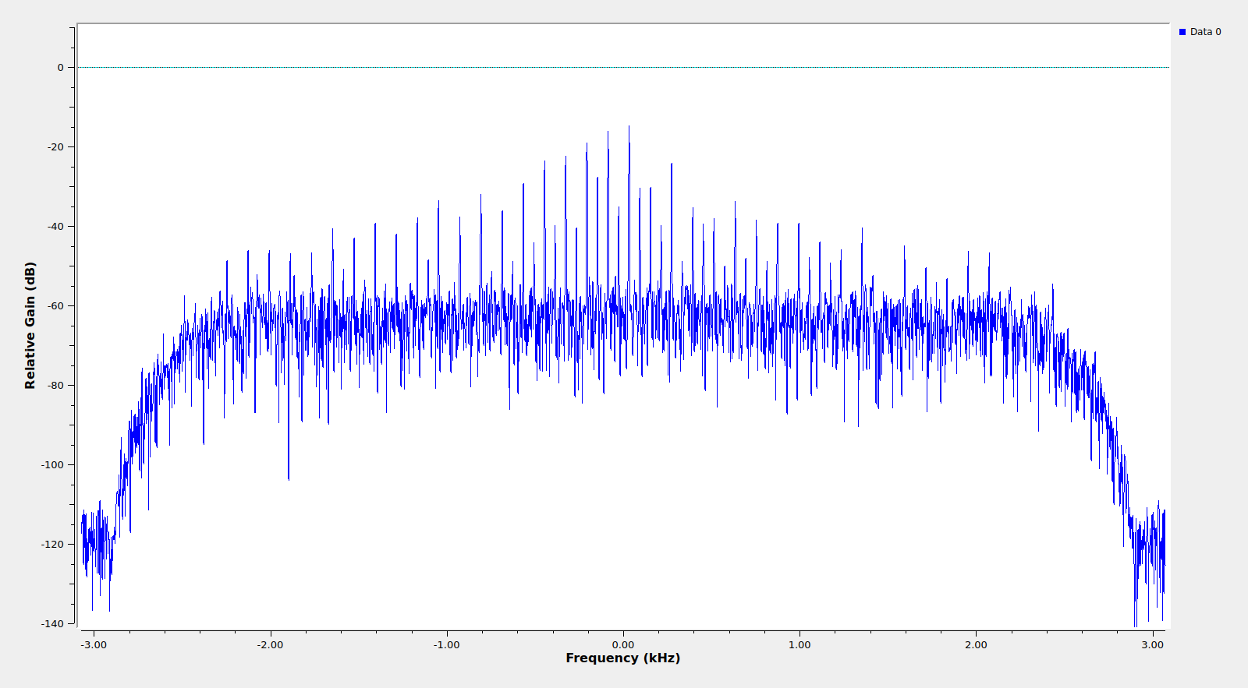
\includegraphics[width=1\linewidth]{figures/GNU-Obs1.png}}
\caption{Tianwen-1 carrier spectra. The CW carrier frequency is set to be at 0\,Hz in this plot.}
\label{fig:Tianwen-1}
\end{figure}
%

The first step in the investigation of this problem done by the GNU-Radio team was to point the ATA at different space crafts to verify that this problem is within the ATA signal path. Targets that were tested were Tianwen-1 (check NASA horizon for RA and DEC) at 8425 MHz, Mars at 8425 MHz (sometimes but not always orbiters can be seen). Also around 2250 MHz pointed almost anywhere (for example, the Moon); Earth orbiting satellites will be seen on the dish sidelobes. The modulation was also visible regardless of whether the USRP was set to internal or external clock. All signals coming from the telescope IF showed this problem. The phase modulation effect was common to both USRPs (in which we typically receive 1hx, 1hy, 4gx, 4gy), and since we were able to correlate signals between different antennas and USRPs without problems, this indicated that the phase modulation must be correlated between antennas and polarizations.

The leading hypothesis to explain this problem at this point was that the modulation must happen in the frequency conversion stages of the ATA. To narrow down if the modulation was confined within one antenna tuning (eg. LOA-D) or common to all tunings we performed a test observation of \ref{fig:Tianwen-1} with following modification. We used antenna 1C and changed the default IF tuning output from tuning D to tuning C and we used antenna 4G with the default IF tuning D. This allowed us to test if the modulation is caused by any one of the two LOs C or D, or if it is common on both tunings, which would indicate that the modulation might be caused by the down-converting LO2.
The result of this measurement showed that the modulation was present in both tunings, hence we investigated LO2. The modification of this test observation was reverted and all antenna IF signals for the GNU-Radio USRPs were provided from tuning D again.

To investigate if LO2 is the cause of the modulation we then replaced the signal generator providing the LO2 local oscillator signal for the ATA frequency conversion stage with the, at that time, unused LOC and observed another spacecraft carrier signal. \textit{Tianwen-1} could not be used, as it was not visible at this time. Figure \ref{fig:GNU-Obs2}, shows the acquired spectrum of the carrier CW signal. One can see two CW carriers at around 2.25 GHz and no 60\,Hz modulation was present.


%
\begin{figure}[h]
\centering{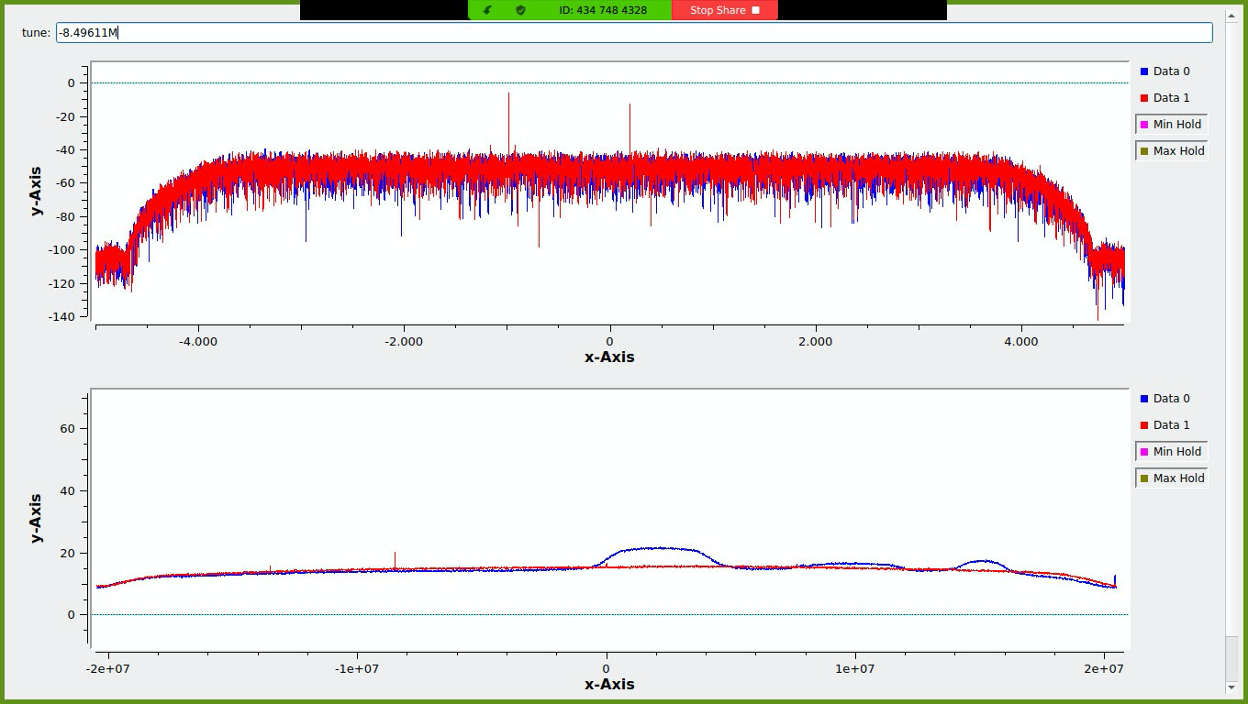
\includegraphics[width=1\linewidth]{figures/GNU-Obs2.png}}
\caption{Spectra of an observed spacecraft carrier. The bottom plot shows the spectra with a frequency span of approximately 40\,MHz and the top plot shows the spectra with a frequency span approximately 8\,KHz. Note that the spacecraft carrier signal in the tip plot is not set exactly to be in the center.  }
\label{fig:GNU-Obs2}
\end{figure}
%

After confirming that the cause of the observed modulation was LO2, we started investigating the LO signal generation, phase stability, time reference and wiring. In the next chapters we describe this investigation in more detail, starting with a description of the test equipment and measurement setup.



%----------------------------------------------------------------------------------------
\section{Measurement Setup}
\label{sec:2}
% ----------------------------------------------------------------

This section describes the setup and hardware used to measure the phase noise and FM modulation of the signal generators which are used to provide the local oscillator signal to the ATA frequency conversions stages.
All measurements have been performed with the Field Fox \href{https://www.keysight.com/en/pdx-x201933-pn-N9938A/fieldfox-handheld-microwave-spectrum-analyzer-265-ghz?pm=spc&nid=-32495.1150527&cc=US&lc=eng}{N9938A} spectrum analyzer and the \href{https://www.rohde-schwarz.com/us/product/nrp_s_sn-productstartpage_63493-99587.html}{NRP-18S} power meter. 

We used to two configuration for the spectrum analyzer, a narrow band (10\,Hz frequency span) and a wide band (500\,Hz frequency span) configuration. The exact settings fo the spectrum analyzer for both configurations are shown in Table \ref{tab:spectrumanalyzer}.


\begin{table}[H]
\caption{Spectrum analyzer settings.} % title name of the table
\centering
\begin{tabular}{l | l|l} \hline\hline
Description & Settings Wide Band & Settings Narrow Band 
\\ [0.5ex]
\hline % inserts single-line
Resolution			& 1001 points 	& 1001 points\\
$center{\rm{freq}}$		& 16.012\,GHz 	& 16.012\,GHz\\
$span$				& 500\,Hz 		& 10\,Hz\\
RBW					& 1\,Hz 		& 1\,Hz\\
VBW		 			& 1\,Hz 		& 1\,Hz\\
Attenuator				& Auto 		& Auto\\
File Format			& .csv 		& .csv\\
Average             		& 10 			& 10\\
\hline 
\end{tabular}
\label{tab:spectrumanalyzer}
\end{table}




 
The various test setups used to measure the phase noise and 60\,Hz modulation are shown in Figure \ref{fig:measurement_setup_overview}. Note that in oder to pin point the problem of the phase noise and 60\,Hz modulation, we also used different combinations of these test setups. All of these measurements however have in common that the spectrum analyzer was always locked to the same 10\,MHz reference as the to be tested signal generator. The drift between the internal oscillator of spectrum analyzer and the oscillator of the to be tested signal generator was so significant that no meaningful measurement was possible without locking them together. In test setups where no external 10\,MHz was present, the spectrum analyzer was connected to the 10\,MHz ref output of the to be testes signal generator directly. 




%
\begin{figure}[H]
\centering{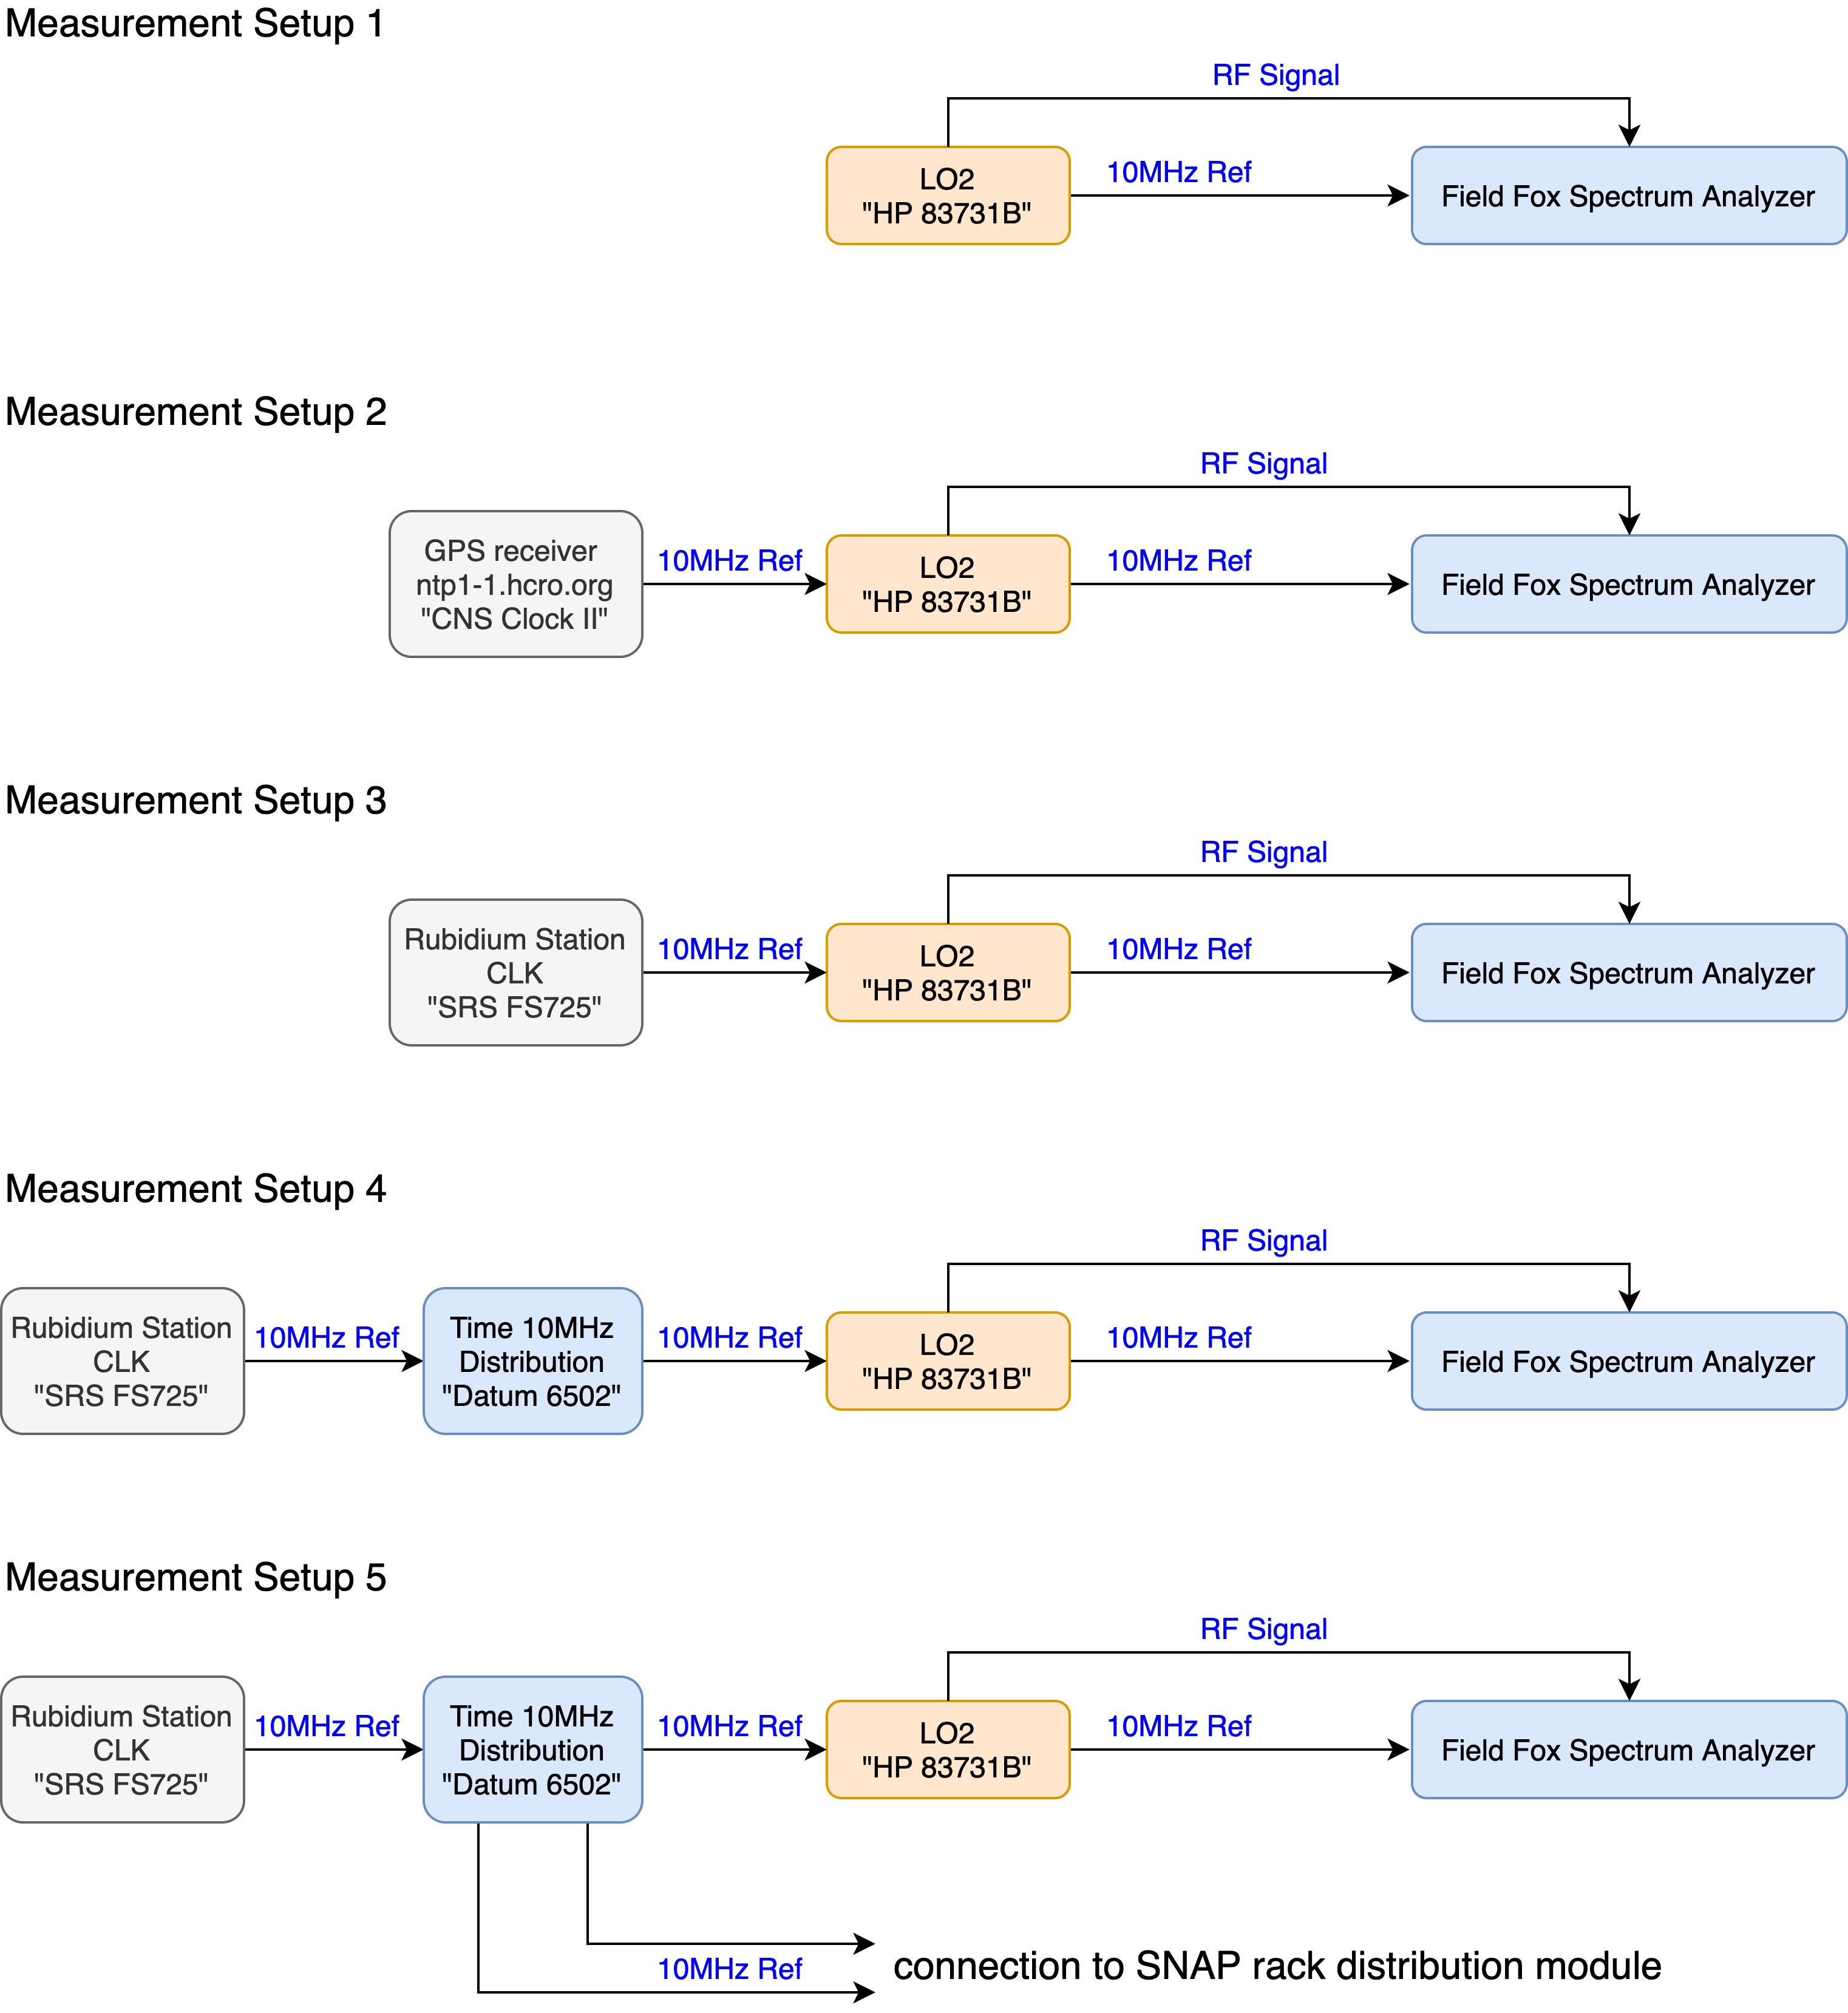
\includegraphics[width=0.99\linewidth]{figures/Measurement_setup_overview.png}}
\caption{Shows the summary of the different measurement setups used to debug the 60\,Hz phase modulation of the local oscillators.}
\label{fig:measurement_setup_overview}
\end{figure}
%






\newpage
%----------------------------------------------------------------------------------------
\section[LO Phase Noise and Spur Measurement]{Local Oscillator Phase Noise and FM Modulation Measurement}
\label{sec:3}
% ----------------------------------------------------------------
\subsection{Initial Investigation}

The first test was done with the existing setup and wiring, where we connected the spectrum analyzer to the output of LO2 and measured the spectra with a span of 500\,Hz. This spectra is shown in Figure \ref{fig:LO2-HP-83731B-original}, one can see strong spurs at 60\,Hz, 120\,Hz, and 180\,Hz which are consistent with the phase modulation observed by the GNU-Radio team, described in Section \ref{sec:1}. During some more tests we discovered that the level of the spurs change, when modifying the 10\,MHz ref wiring within the LO rack. Moreover, half of the equipment got its main connection from sockets of the neighboring racks. At this point we decided to clean up the entire wiring of the LO rack and also go over all cables that distribute the 10\,MHz and 1PPS signal to other racks. 

%
\begin{figure}[H]
\centering{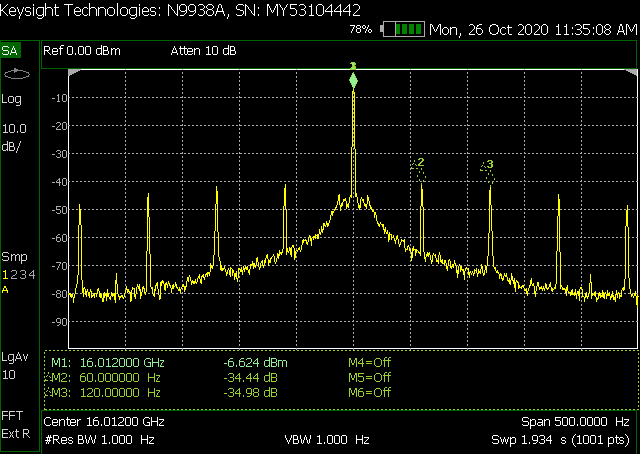
\includegraphics[width=0.9\linewidth]{figures/LO2-HP-83731B-original.png}}
\caption{Initial measured spectra of local oscillator 2 which was used to drive the down-conversion stage of the RFCBs. The strong spurs at 60\,Hz and its harmonics correlate with the observed phase modulation seen in the GNU-Radio observation described in Section \ref{sec:1}. }
\label{fig:LO2-HP-83731B-original}
\end{figure}
%

The before and after picture of the LO rack is shown in Figure \ref{fig:before-after}. In the process of cleaning up the rack we installed a power distribution unit at the bottom of the rack, which now supplies all hardware installed within that rack. We also removed a number of 10\,MHz and 1PPS reference cables that were connected to the distribution units in the LO rack, but weren't connected to equipment at the other end. We also discovered that the LO signal cables going from the signal generator to the LO distribution units in the RFCB rack were too short and have been extended using lower quality cables and SMA connectors. Moreover, some of these connections were not tighten correctly. The operational frequency of LO2 is approximately 16\,GHz whereas for LOA-D depending on the selected sky frequency the LO frequency ranges from 16\,GHz up to 28\,GHz.


%
\begin{figure}[H]
\centering{\includegraphics[width=0.9\linewidth]{figures/before-after.png}}
\caption{Shows the rear side of the LO rack before and after we cleaned up the wiring.}
\label{fig:before-after}
\end{figure}
%



After the cleanup and rewiring of the LO rack we measured the output of LO2 again and compared it to the original measurement seen in Figure \ref{fig:LO2-HP-83731B-original}. The measured spectra of LO2 after the clean up is shown in Figure \ref{fig:LO2-HP-83731B-after-rack-cleanup}, one can see that the power level of the 60\,Hz spur is reduced and the 120\,Hz spur is completly gone. At this point in time we used LO2 again as the down-converting LO in the ATA signal path and repeated the original observation of a spacecraft carrier signal, which resulted in a clean spectrum. 

%
\begin{figure}[H]
\centering{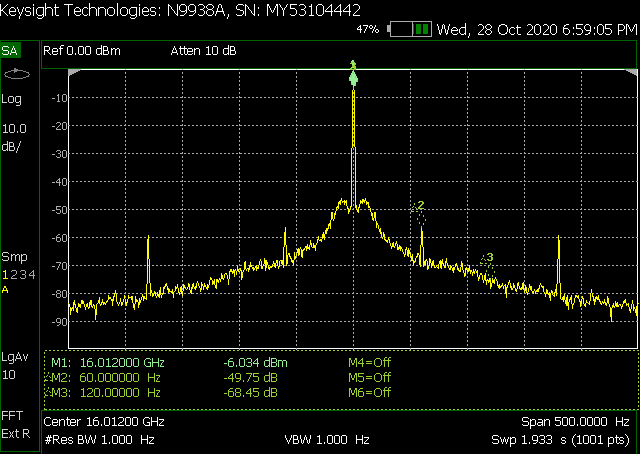
\includegraphics[width=0.9\linewidth]{figures/LO2-HP-83731B-after-rack-cleanup.png}}
\caption{Spectra of the local oscillator 2 output after the LO rack was cleaned up.}
\label{fig:LO2-HP-83731B-after-rack-cleanup}
\end{figure}
%

\subsection{10\,MHz Reference Test}

In order to further understand the impact of the 10\,MHz reference signal wiring we continued to measure the phase noise and spurs of the 5 signal generators that are used as local oscillators for the ATA frequency conversion stage. In order to be independent of any failure modes that might be specific to LO2, we used LOA for the following tests. LOA is an Agilent E8257D analog signal generator. The following spectra were measured using the test setups presented in Section \ref{sec:2} Figure \ref{fig:measurement_setup_overview}.

Each figure consists of the measured spectra and a block diagram of its measurement setup. The first measurement was done to test the output signal of the signal generator when isolated form the rest of the hardware in the LO rack. As one can see in Figure \ref{fig:Measurement-Setup1} practically no spurs are present, which is a good baseline for what the signal generator can provide with respect to phase noise and spurs. We then connected the signal generator to the external 10\,MHz reference of the GPS receiver, the corresponding spectra is shown in Figure \ref{fig:Measurement-Setup2}. One can see that a 60\,Hz and 180\,Hz spur got coupled into the output of the signal generator though its 10\,MHz reference input. 
In the third measurement, we replaced the GPS receiver 10\,MHz reference with the 10\,MHz reference of the SRS F725 Rubidium station clock. The spectra for this setup, presented in Figure \ref{fig:Measurement-Setup3} shows very small spurs and is nearly as clean as the first test with no external 10\,MHz reference present. In the fourth test we added the 10\,MHz distribution module (Datum 6502) and connected it between the output of the station clock and the input of the signal generator. 
%
\begin{figure}[ht!]
\centering{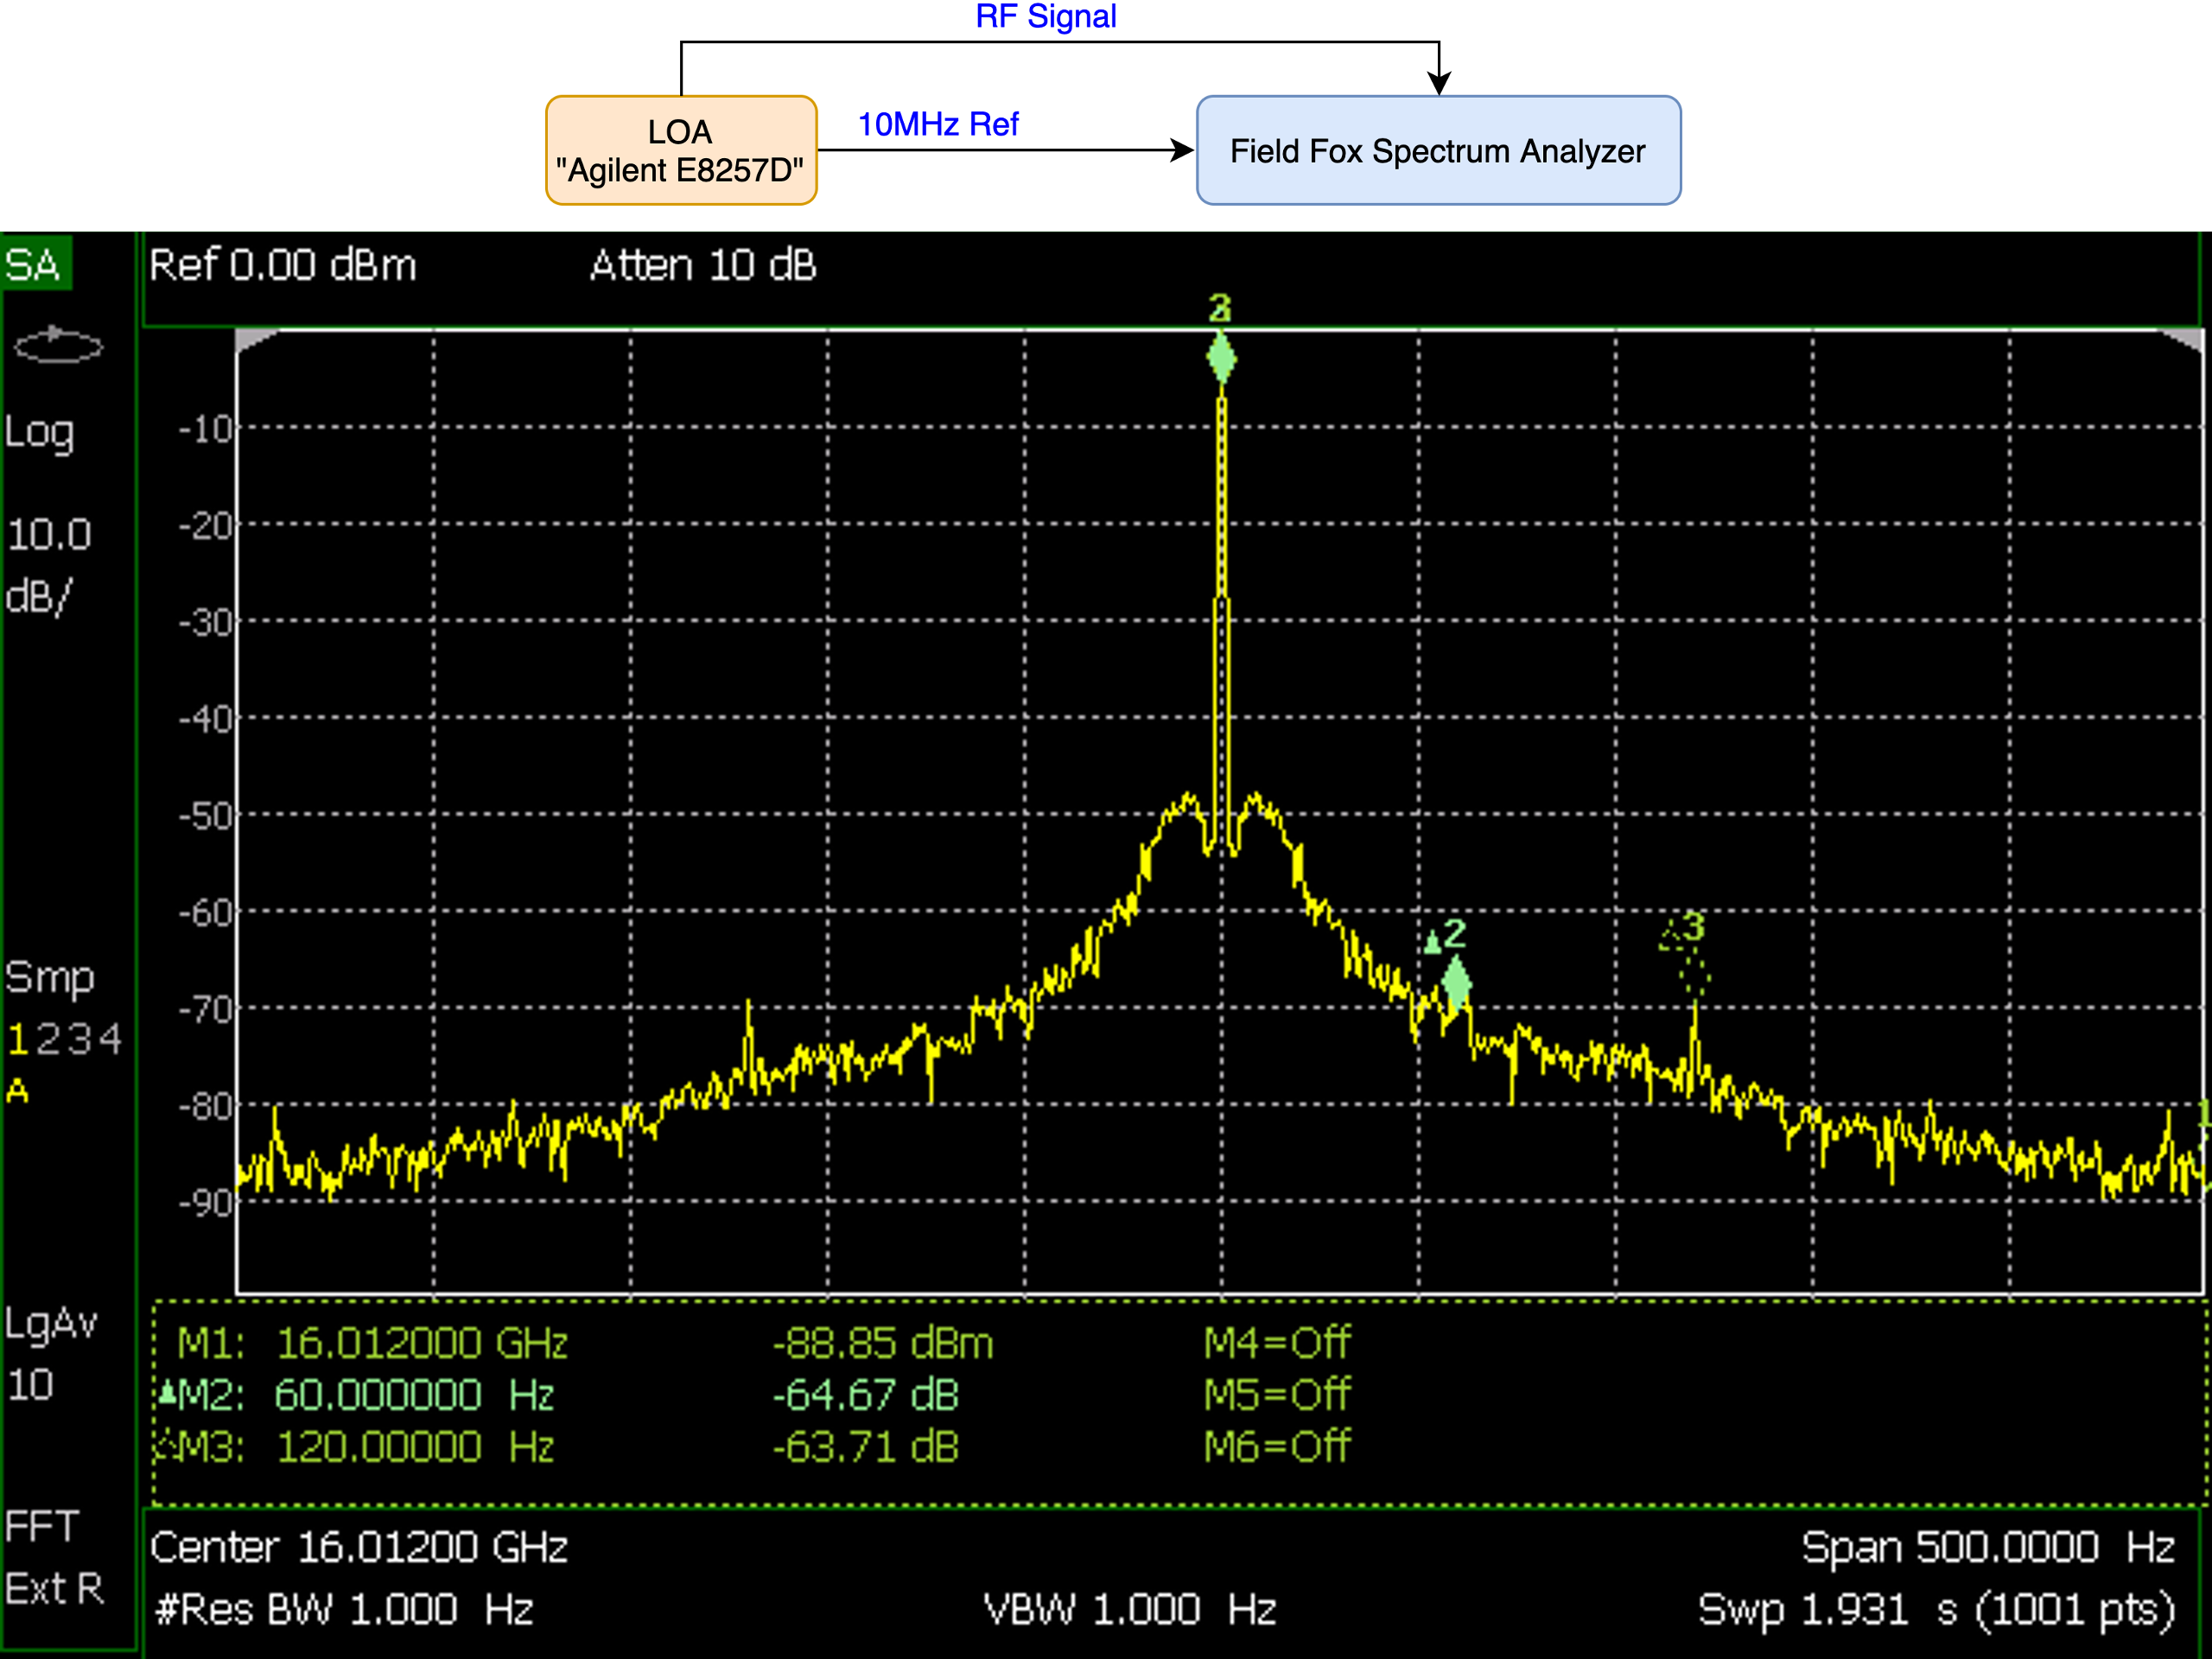
\includegraphics[width=0.8\linewidth]{figures/Measurement-Setup1.png}}
\caption{Spectra of the to be tested LOA, using measurement setup 1.}
\label{fig:Measurement-Setup1}
\end{figure}
%
%
\begin{figure}[ht!]
\centering{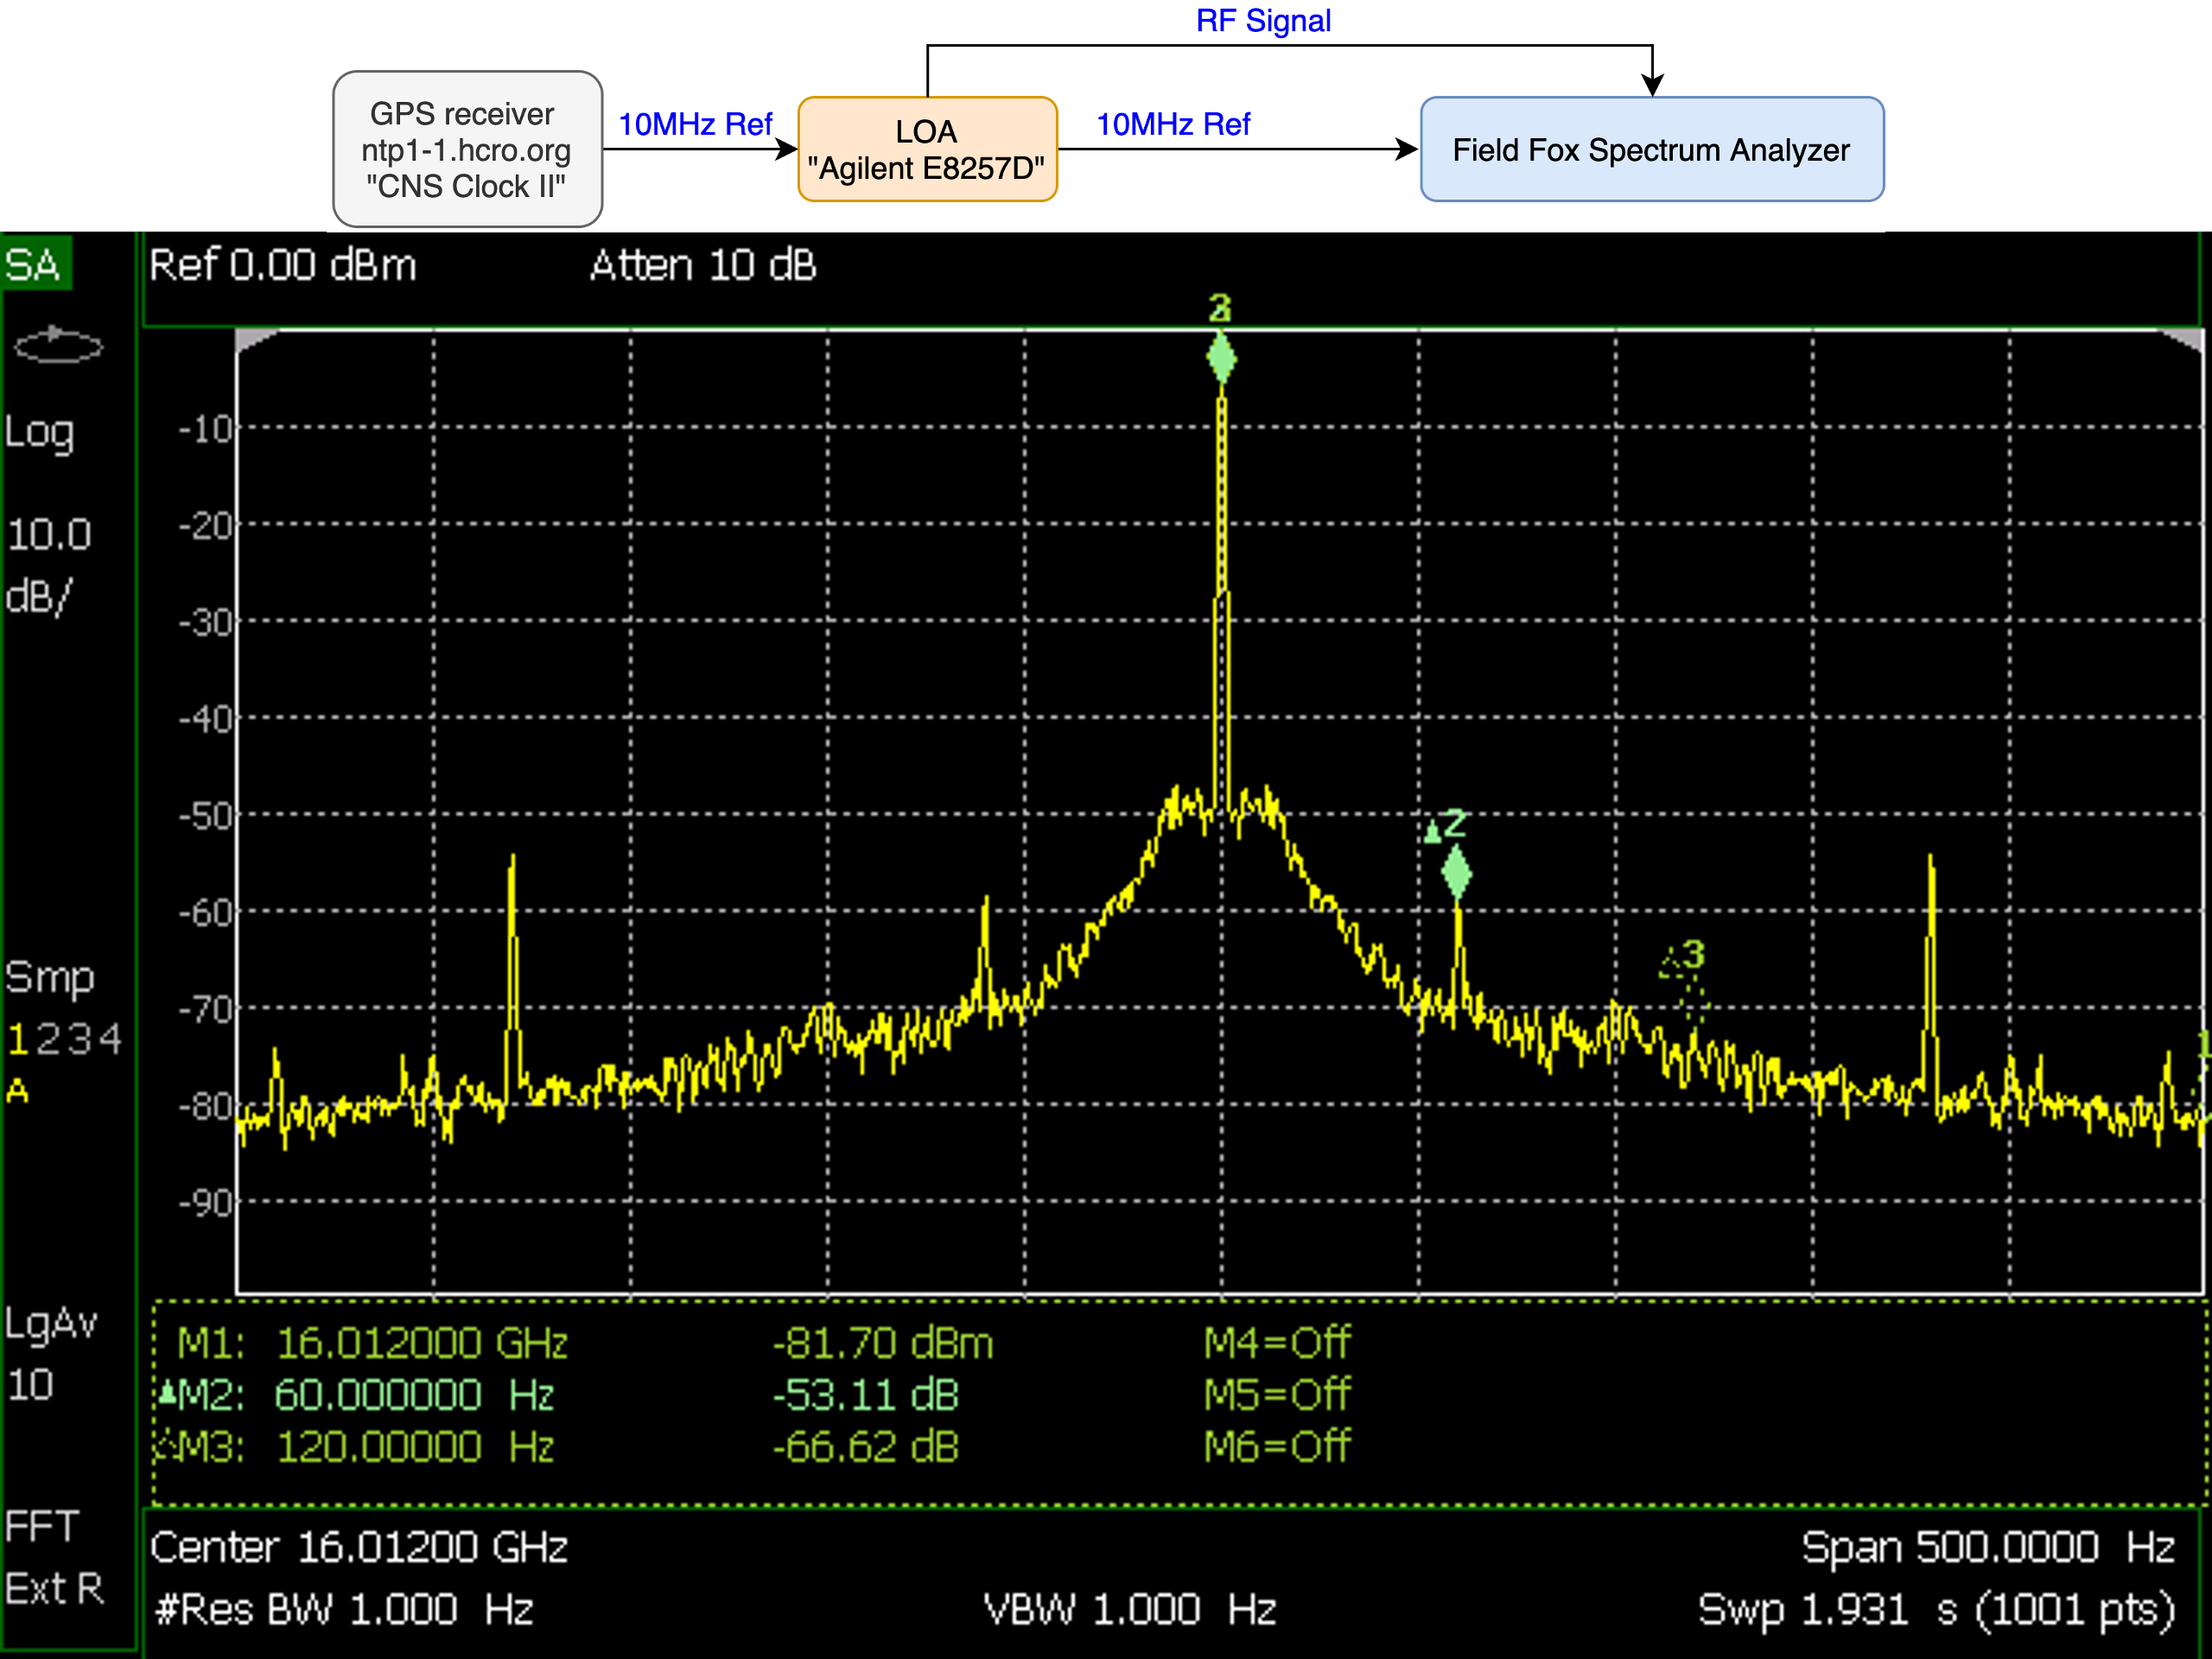
\includegraphics[width=0.8\linewidth]{figures/Measurement-Setup2.png}}
\caption{Spectra of the to be tested LOA, using measurement setup 2.}
\label{fig:Measurement-Setup2}
\end{figure}
%
%
\begin{figure}[ht!]
\centering{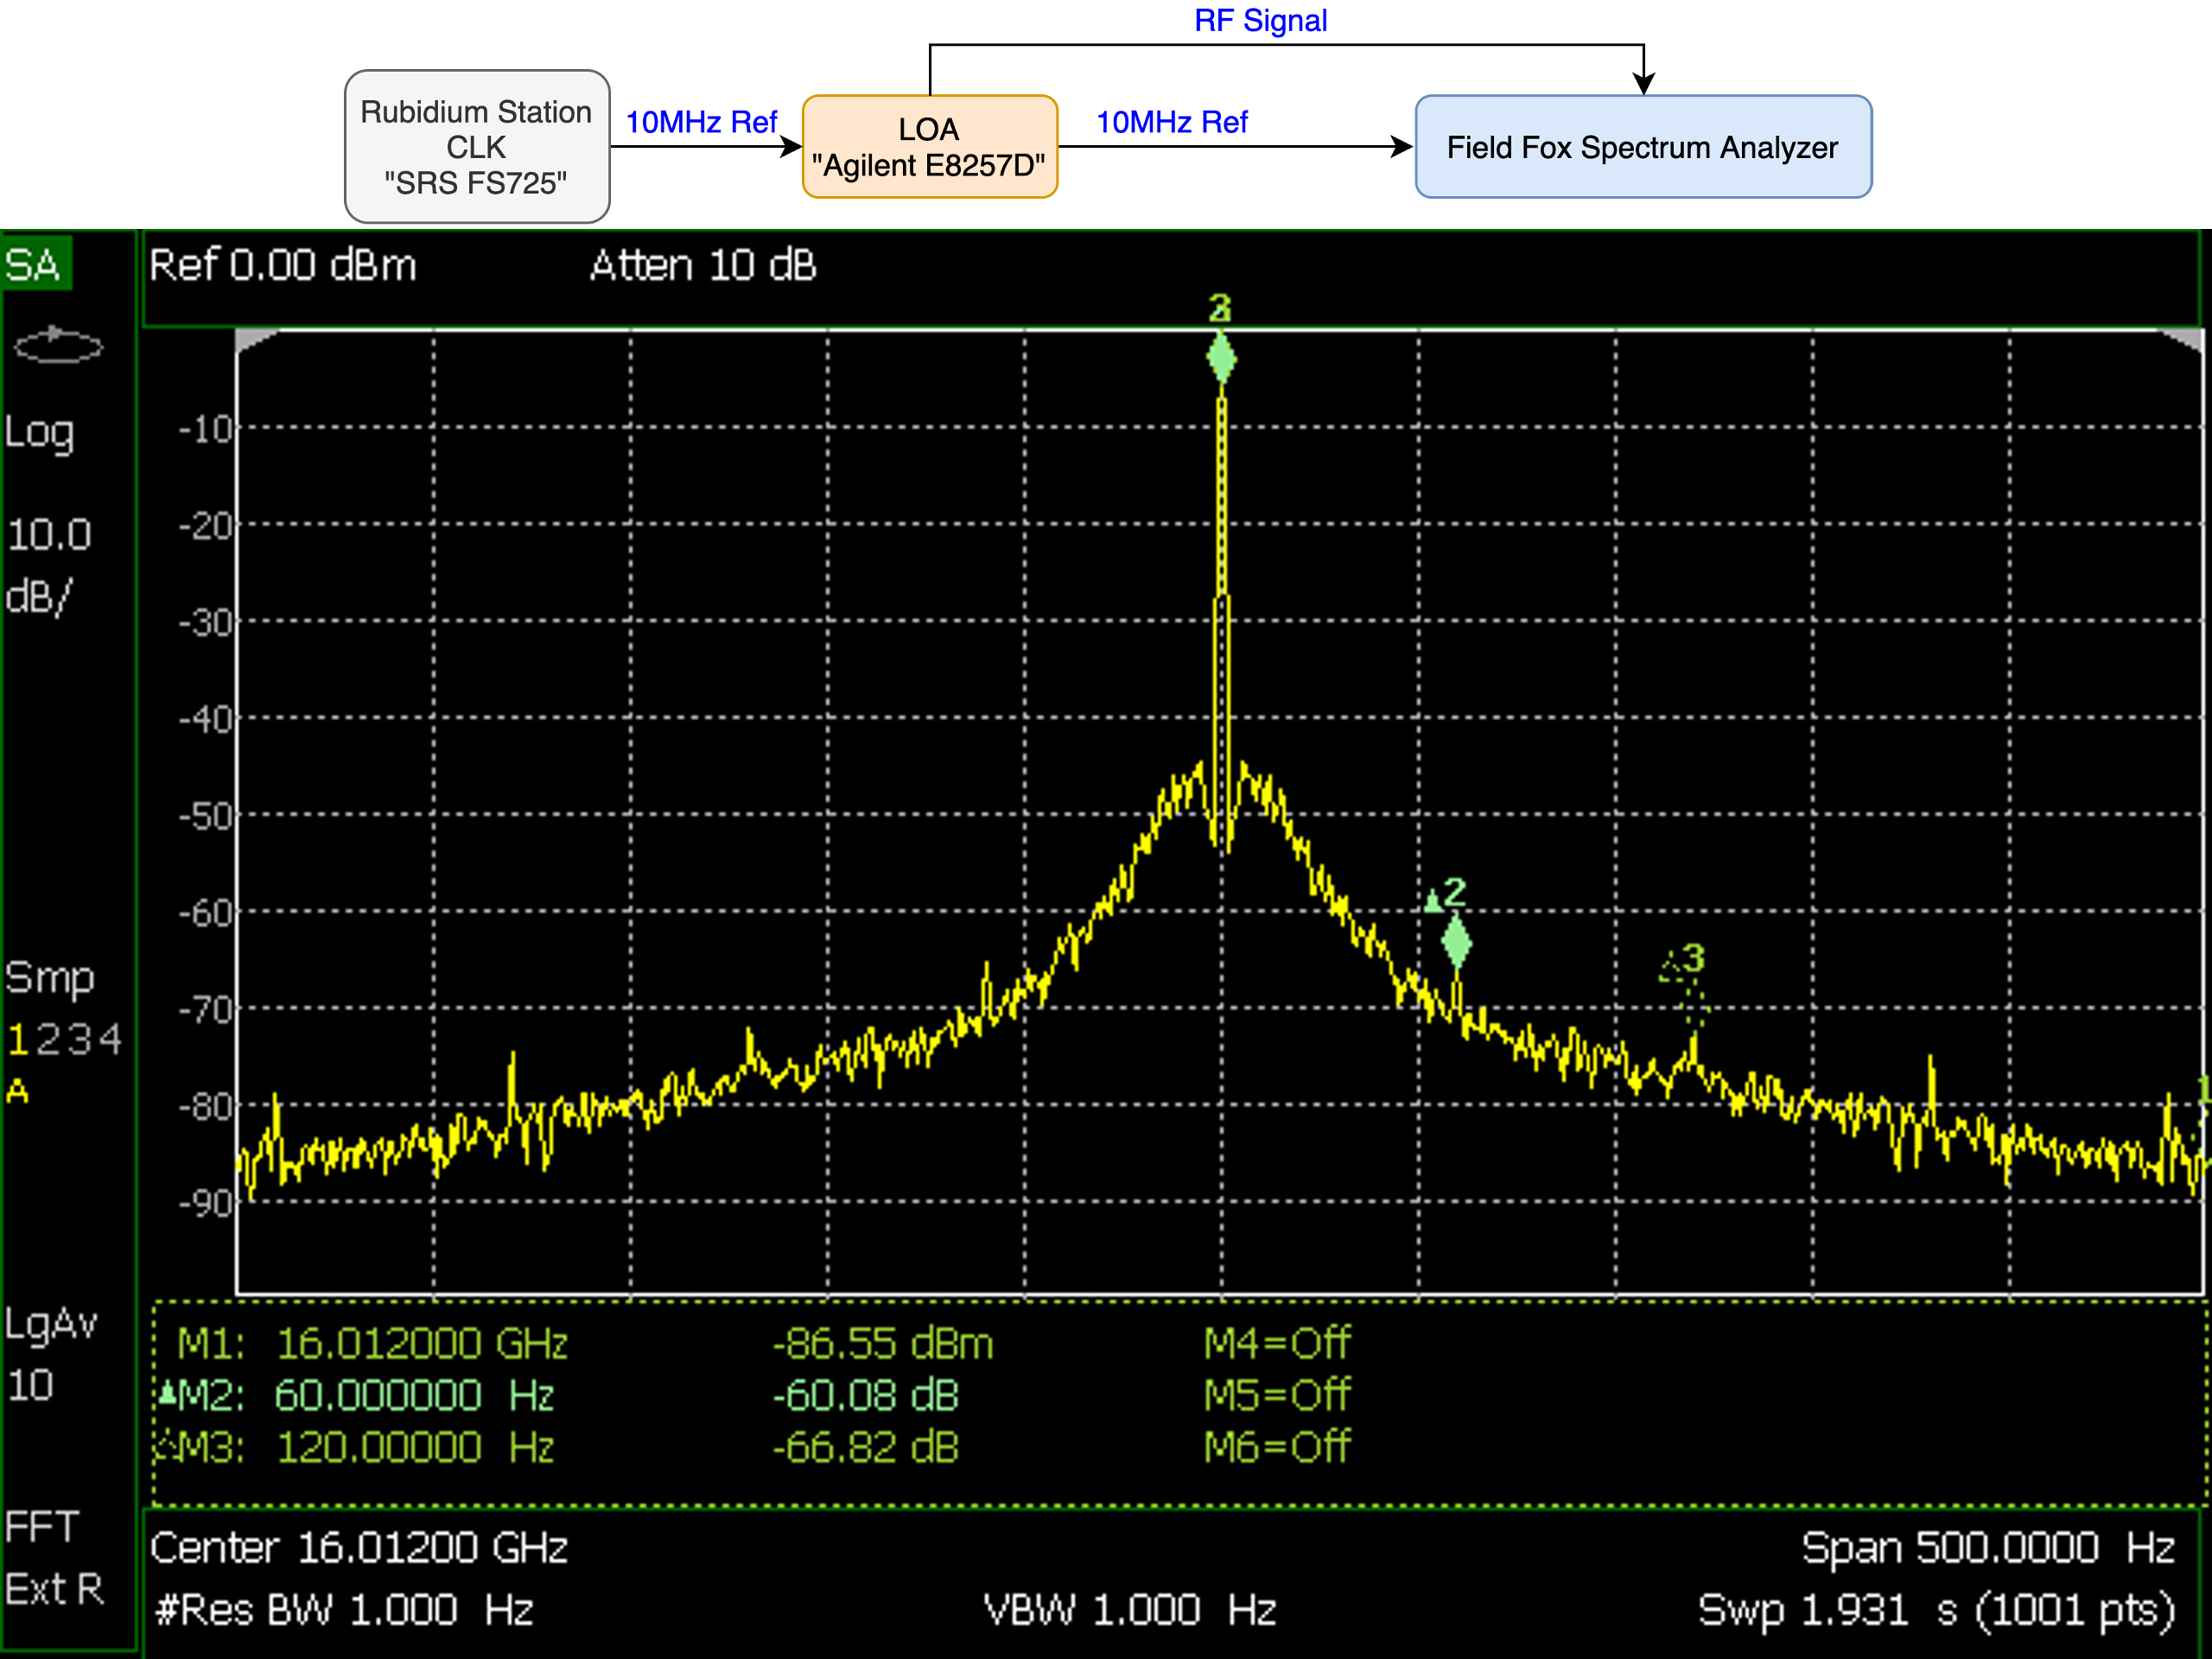
\includegraphics[width=0.8\linewidth]{figures/Measurement-Setup3.png}}
\caption{Spectra of the to be tested LOA, using measurement setup 3.}
\label{fig:Measurement-Setup3}
\end{figure}
%
%
\begin{figure}[ht!]
\centering{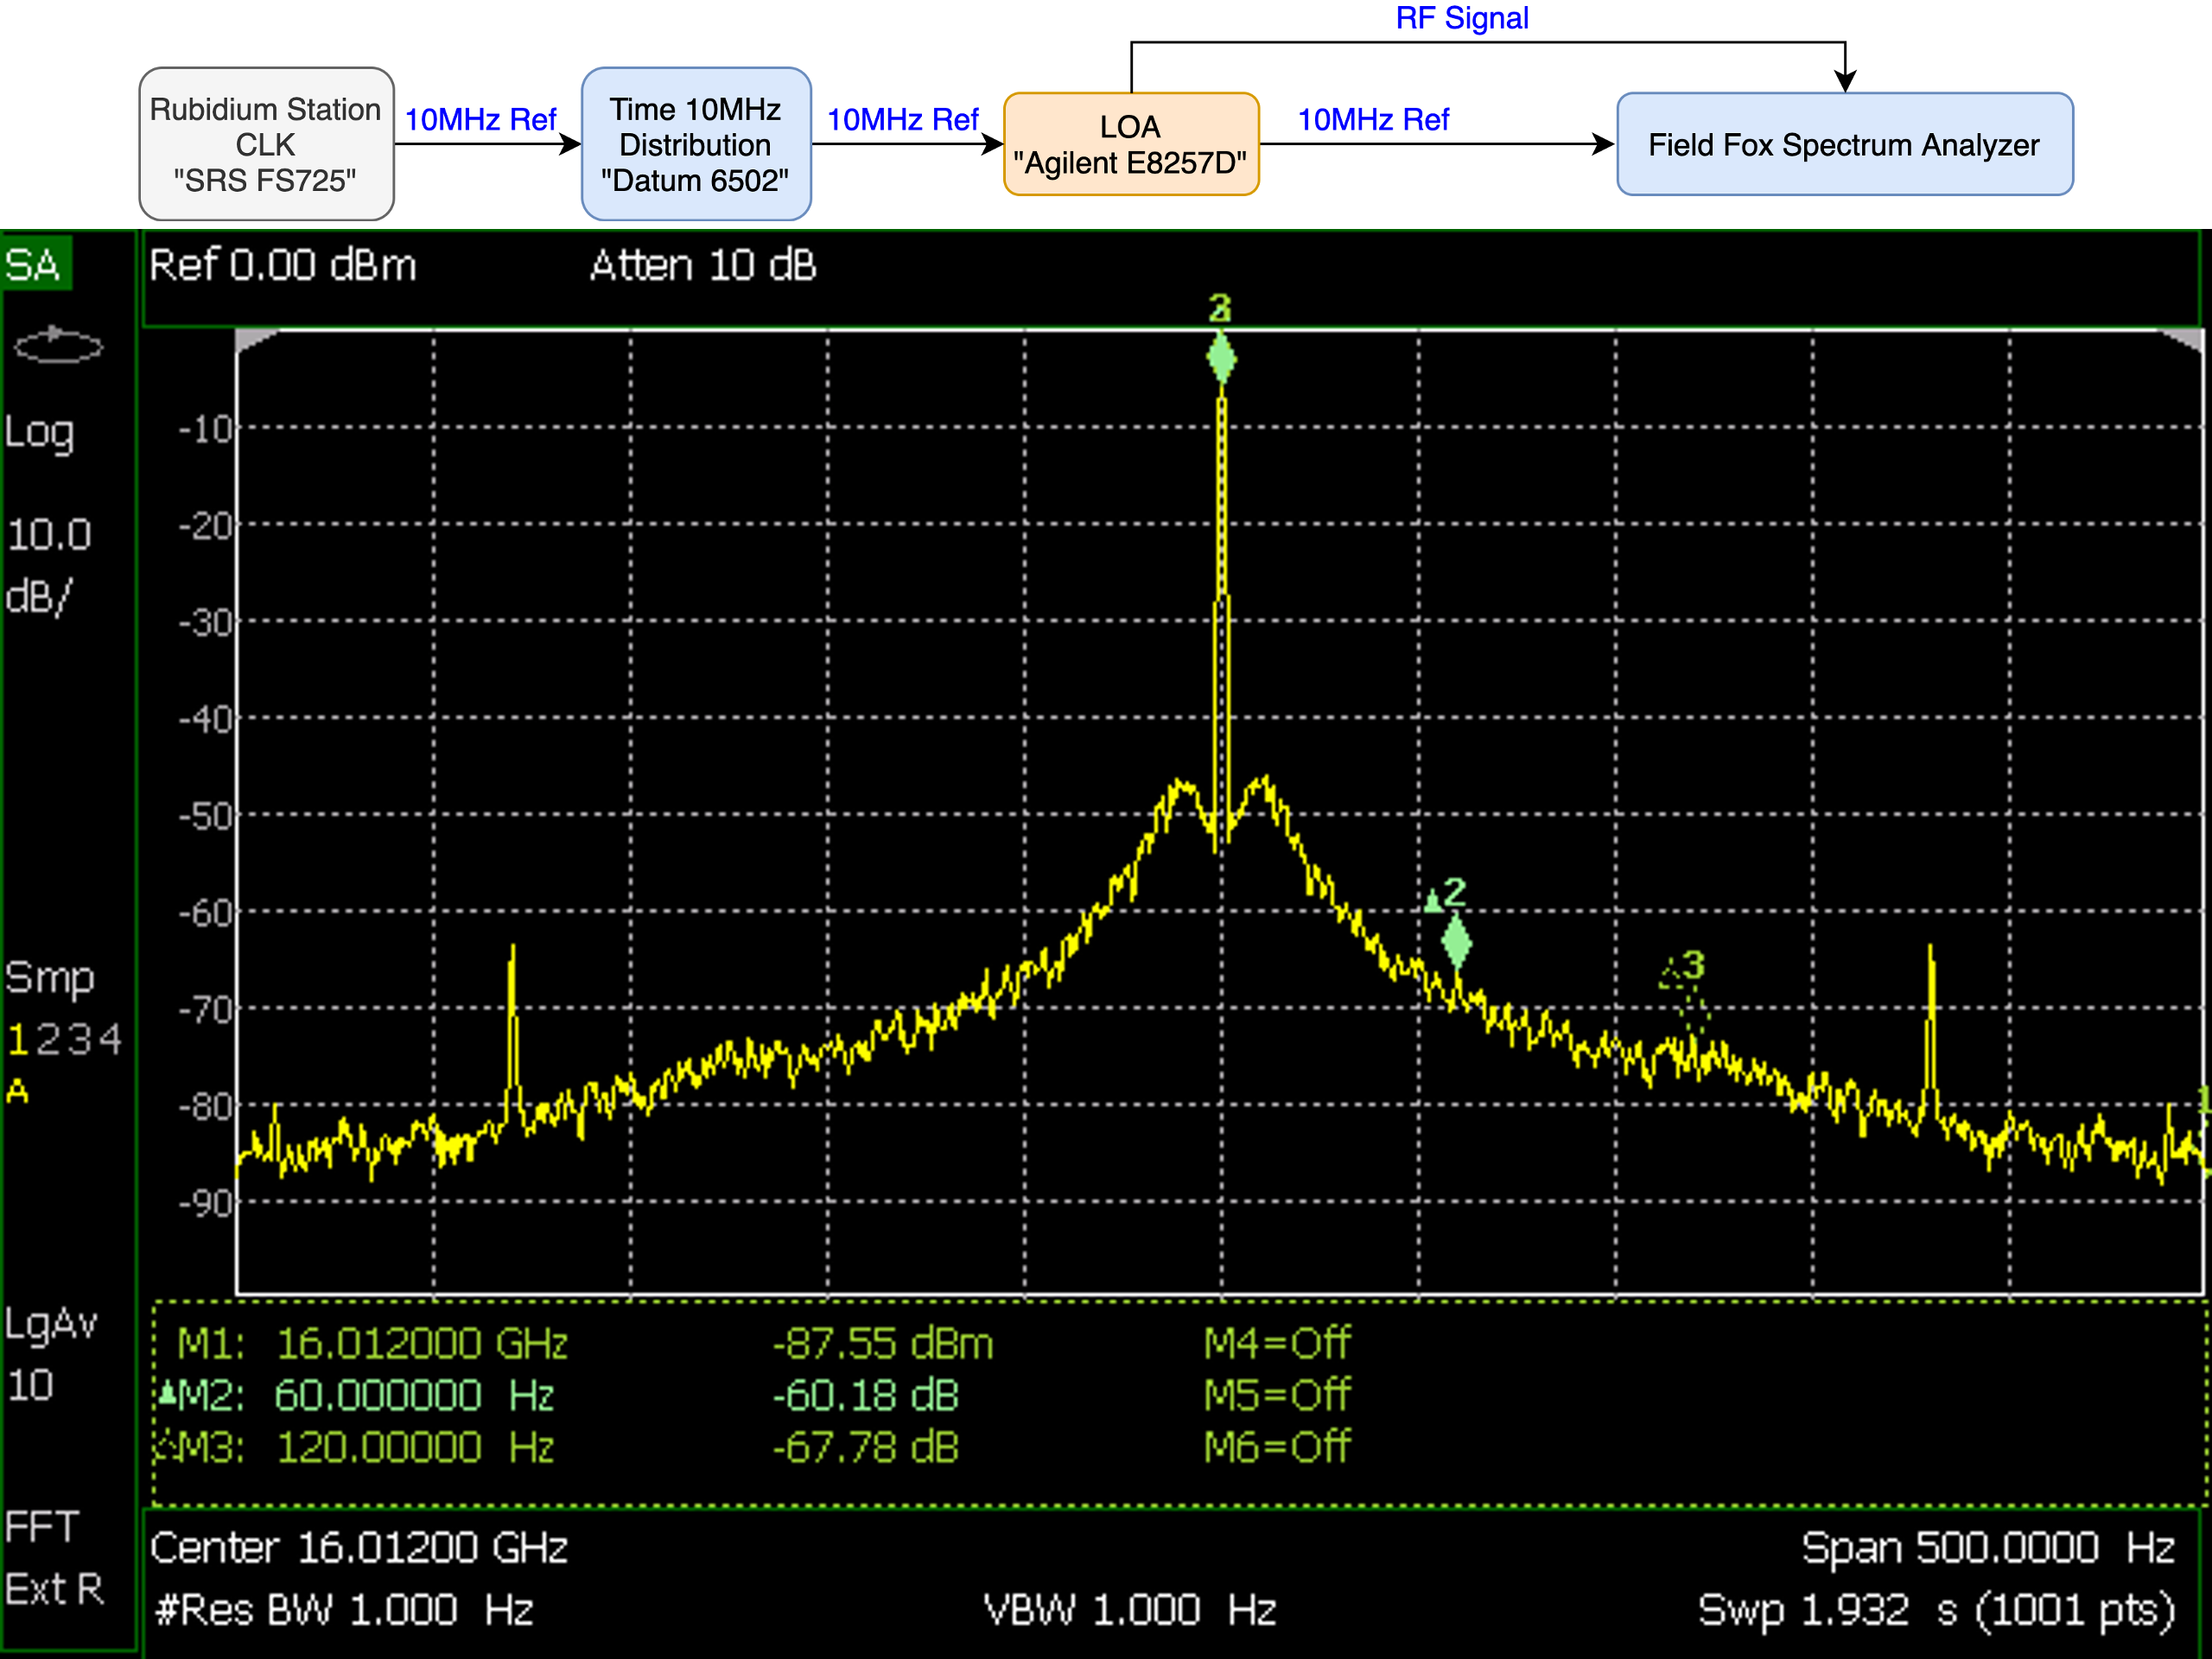
\includegraphics[width=0.8\linewidth]{figures/Measurement-Setup4.png}}
\caption{Spectra of the to be tested LOA, using measurement setup 4.}
\label{fig:Measurement-Setup4}
\end{figure}
%
%
\begin{figure}[ht!]
\centering{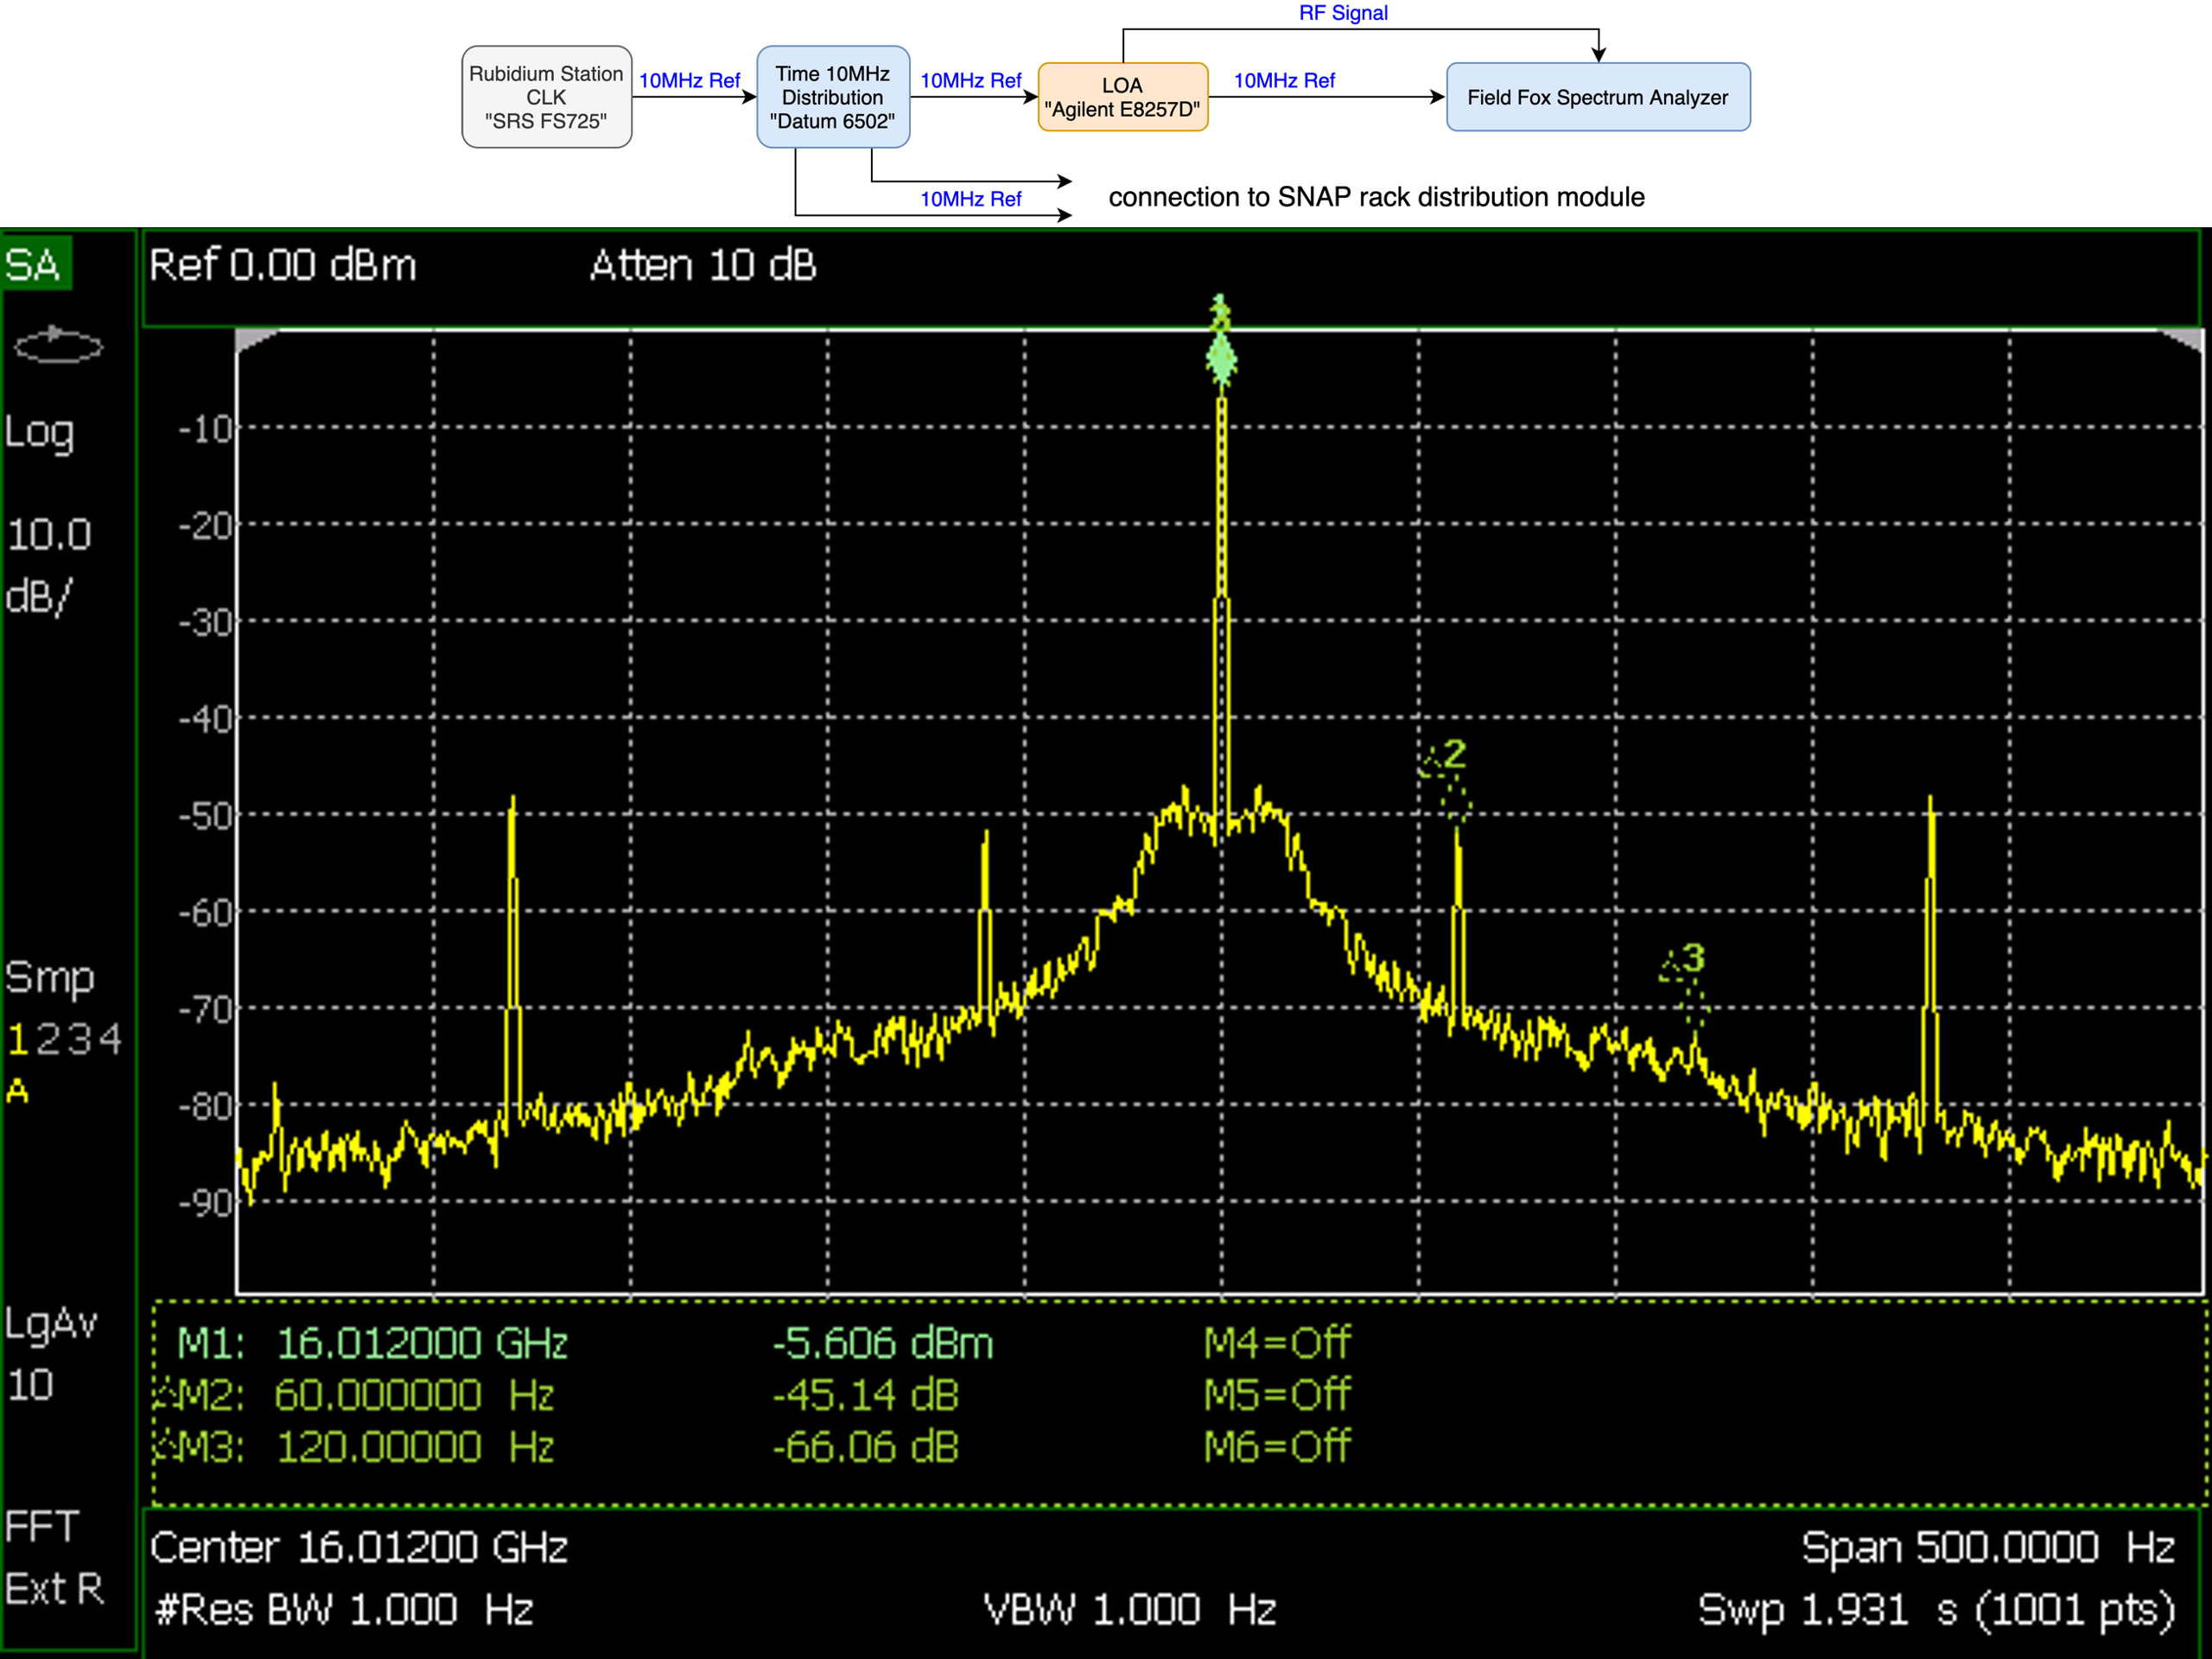
\includegraphics[width=0.8\linewidth]{figures/Measurement-Setup5.png}}
\caption{Spectra of the to be tested LOA, using measurement setup 5.}
\label{fig:Measurement-Setup5}
\end{figure}
%
As one can see in Figure \ref{fig:Measurement-Setup4}, a spur at 180\,Hz appeared.
However, there are still no significant spurs at 60\,Hz or 120\,Hz. In the final setup we also connected the two 10\,MHz distribution cables, which provide the time reference to the DSP hardware in the SNAP / USRP rack. When looking at the spectra for this setup, shown in Figure\ref{fig:Measurement-Setup5}, one can see that the 60\,Hz spur appeared and the 180\,Hz spur increased. 

Based on this experiment we conclude that the cables going to different racks in the SPR contaminate the 10\,MHz reference signal causing spurs to appear in the output of the local oscillators. The exact mechanism of this contamination is at this point in time not fully understood. However, based on the information we gained during this experiment we could modify the wiring of the 10\,MHz reference in a way that minimizes this effect. 

\subsection{Narrow Band Phase Noise Measurement}

As part of the overall phase noise and phase modulation investigation we also looked at the output of the local oscillators with a frequency span of 10\,Hz. However, the smallest RBW and VBW setting possible with our spectrum analyzer is 1\,Hz. Figure \ref{fig:Measurement-Setup1-LOA-10Hz} and \ref{fig:Measurement-Setup1-LO2-10Hz} show the narrow band spectra for LOA and LO2 , respectively. One can see that the overall phase noise for both signal generators is comparable. This is a further indication that LO2 is in working condition and the original phase modulation detected during spacecraft carrier observations were due to the wiring configuration of the LO rack.


%
\begin{figure}[ht!]
\centering{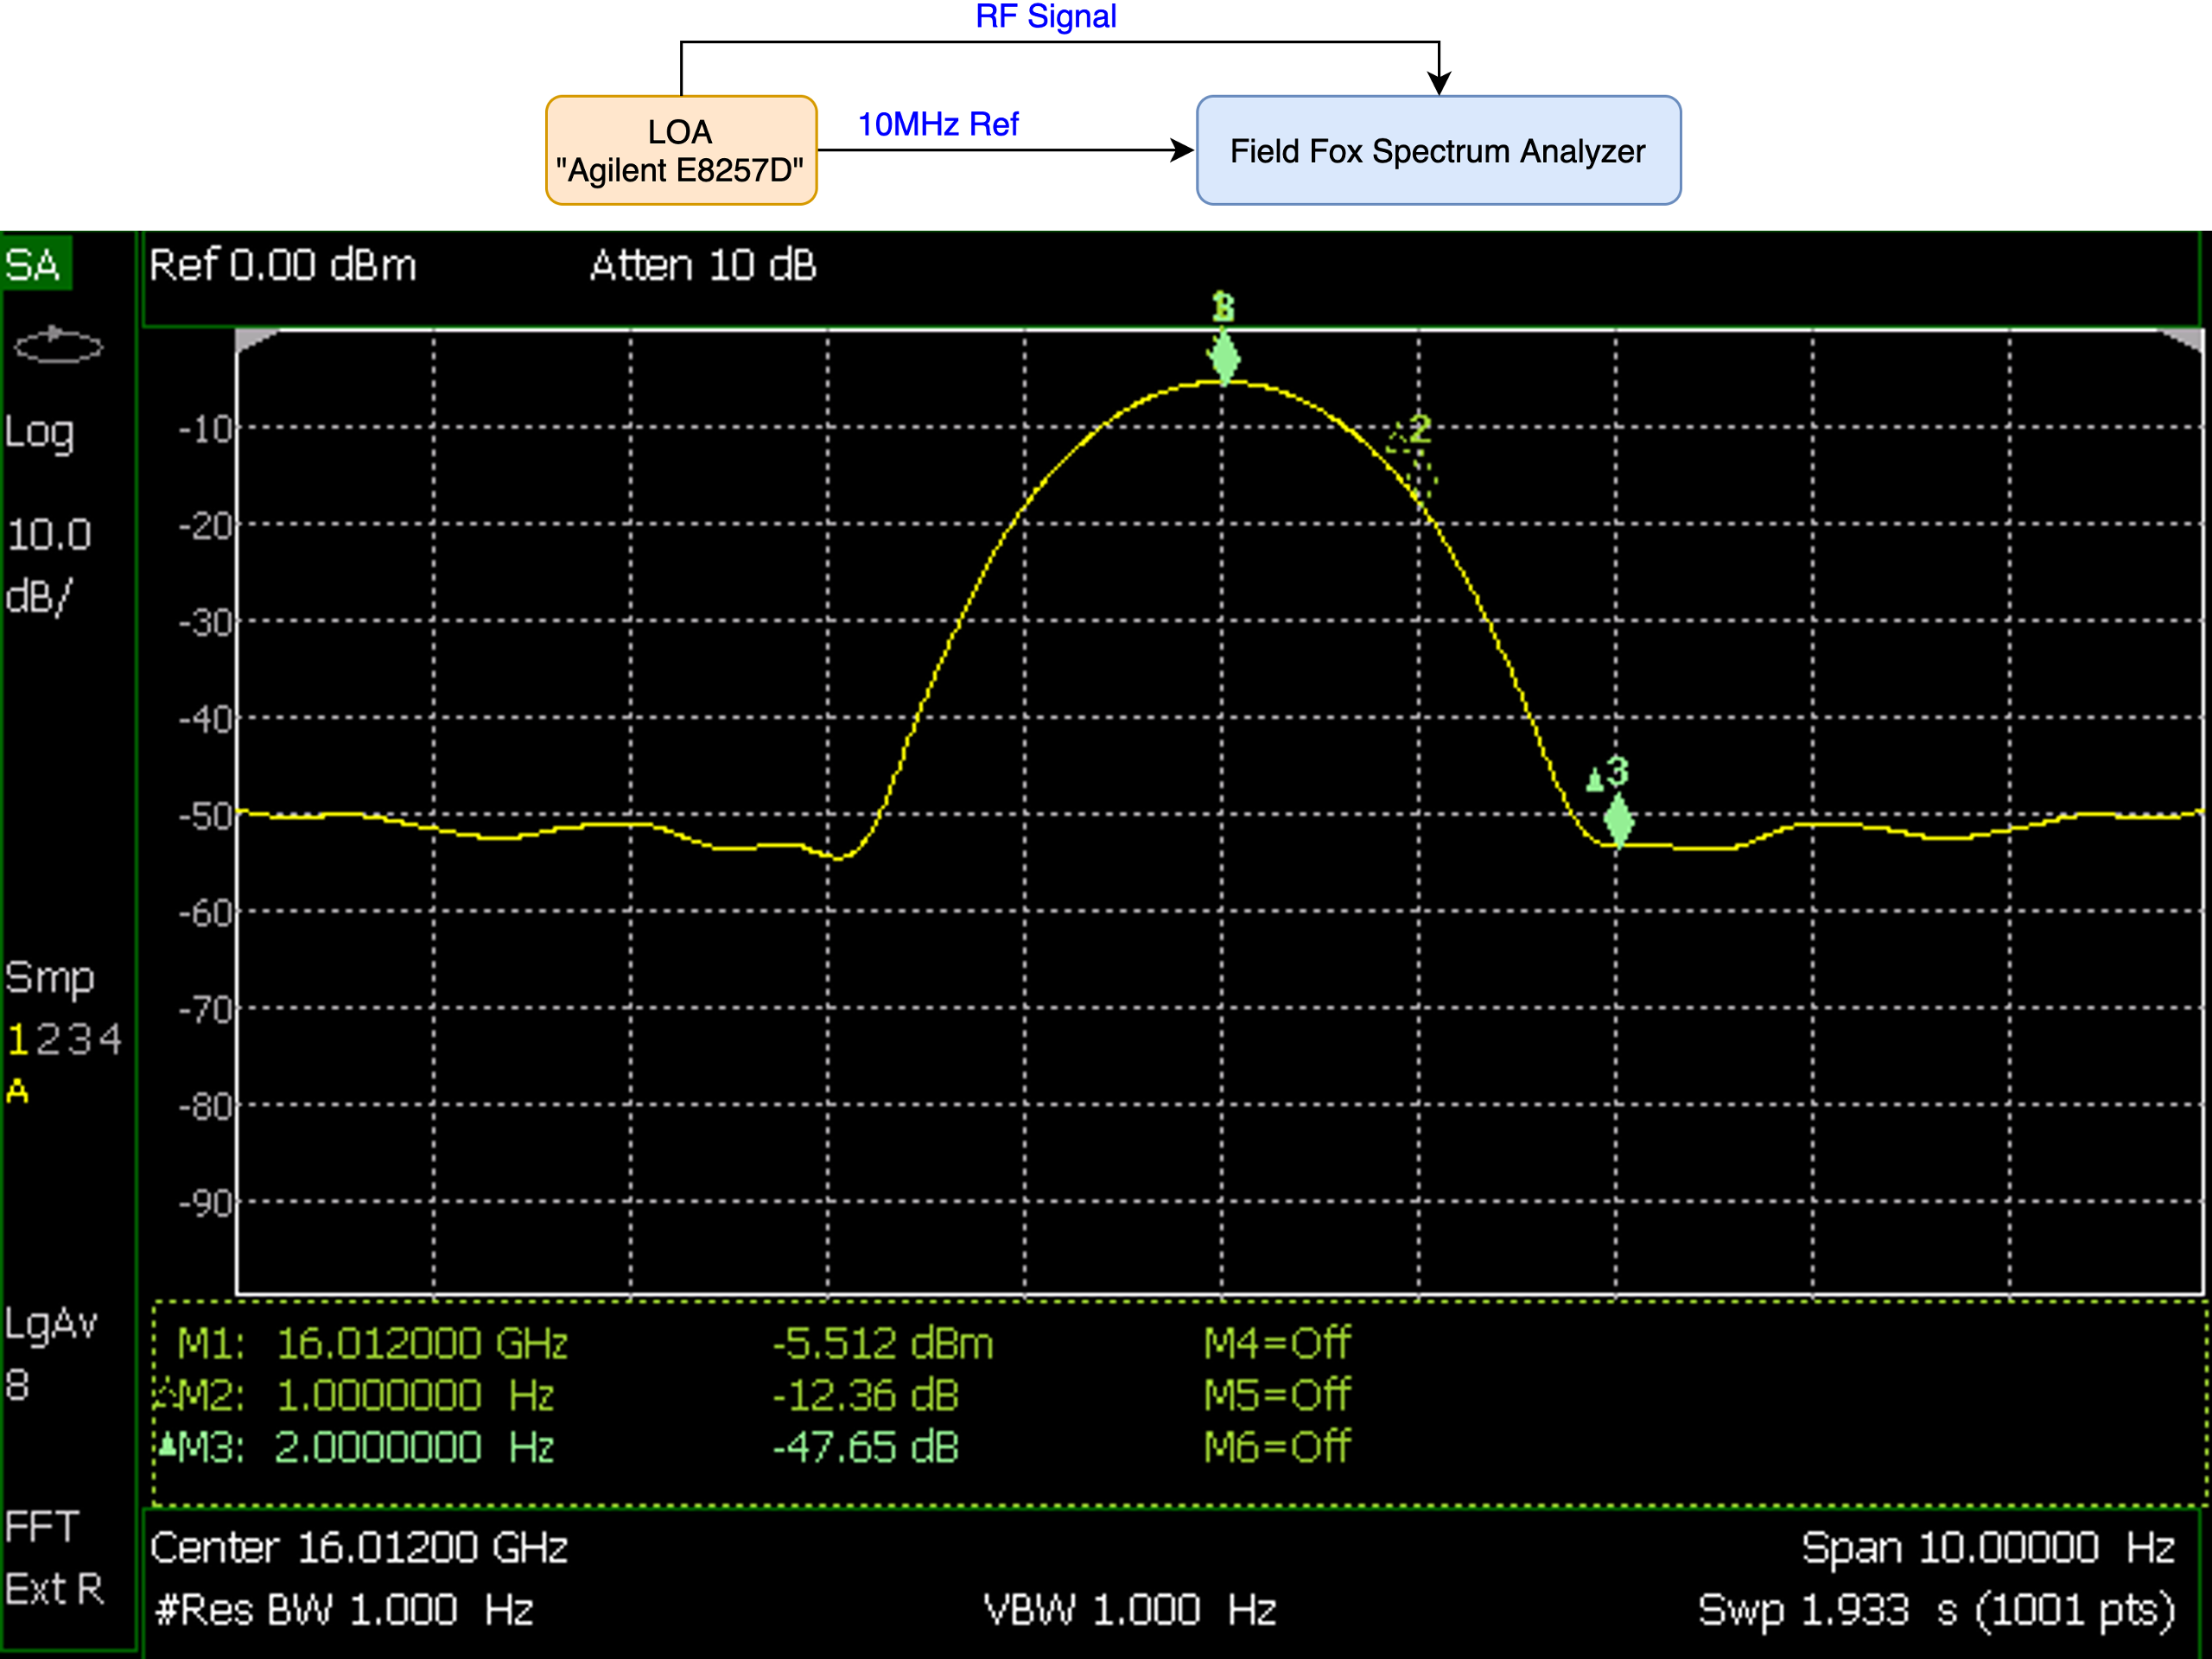
\includegraphics[width=0.8\linewidth]{figures/Measurement-Setup1-LOA-10Hz.png}}
\caption{Narrow band spectra of LOA with a frequency span of 10\,Hz.}
\label{fig:Measurement-Setup1-LOA-10Hz}
\end{figure}
%
%
\begin{figure}[ht!]
\centering{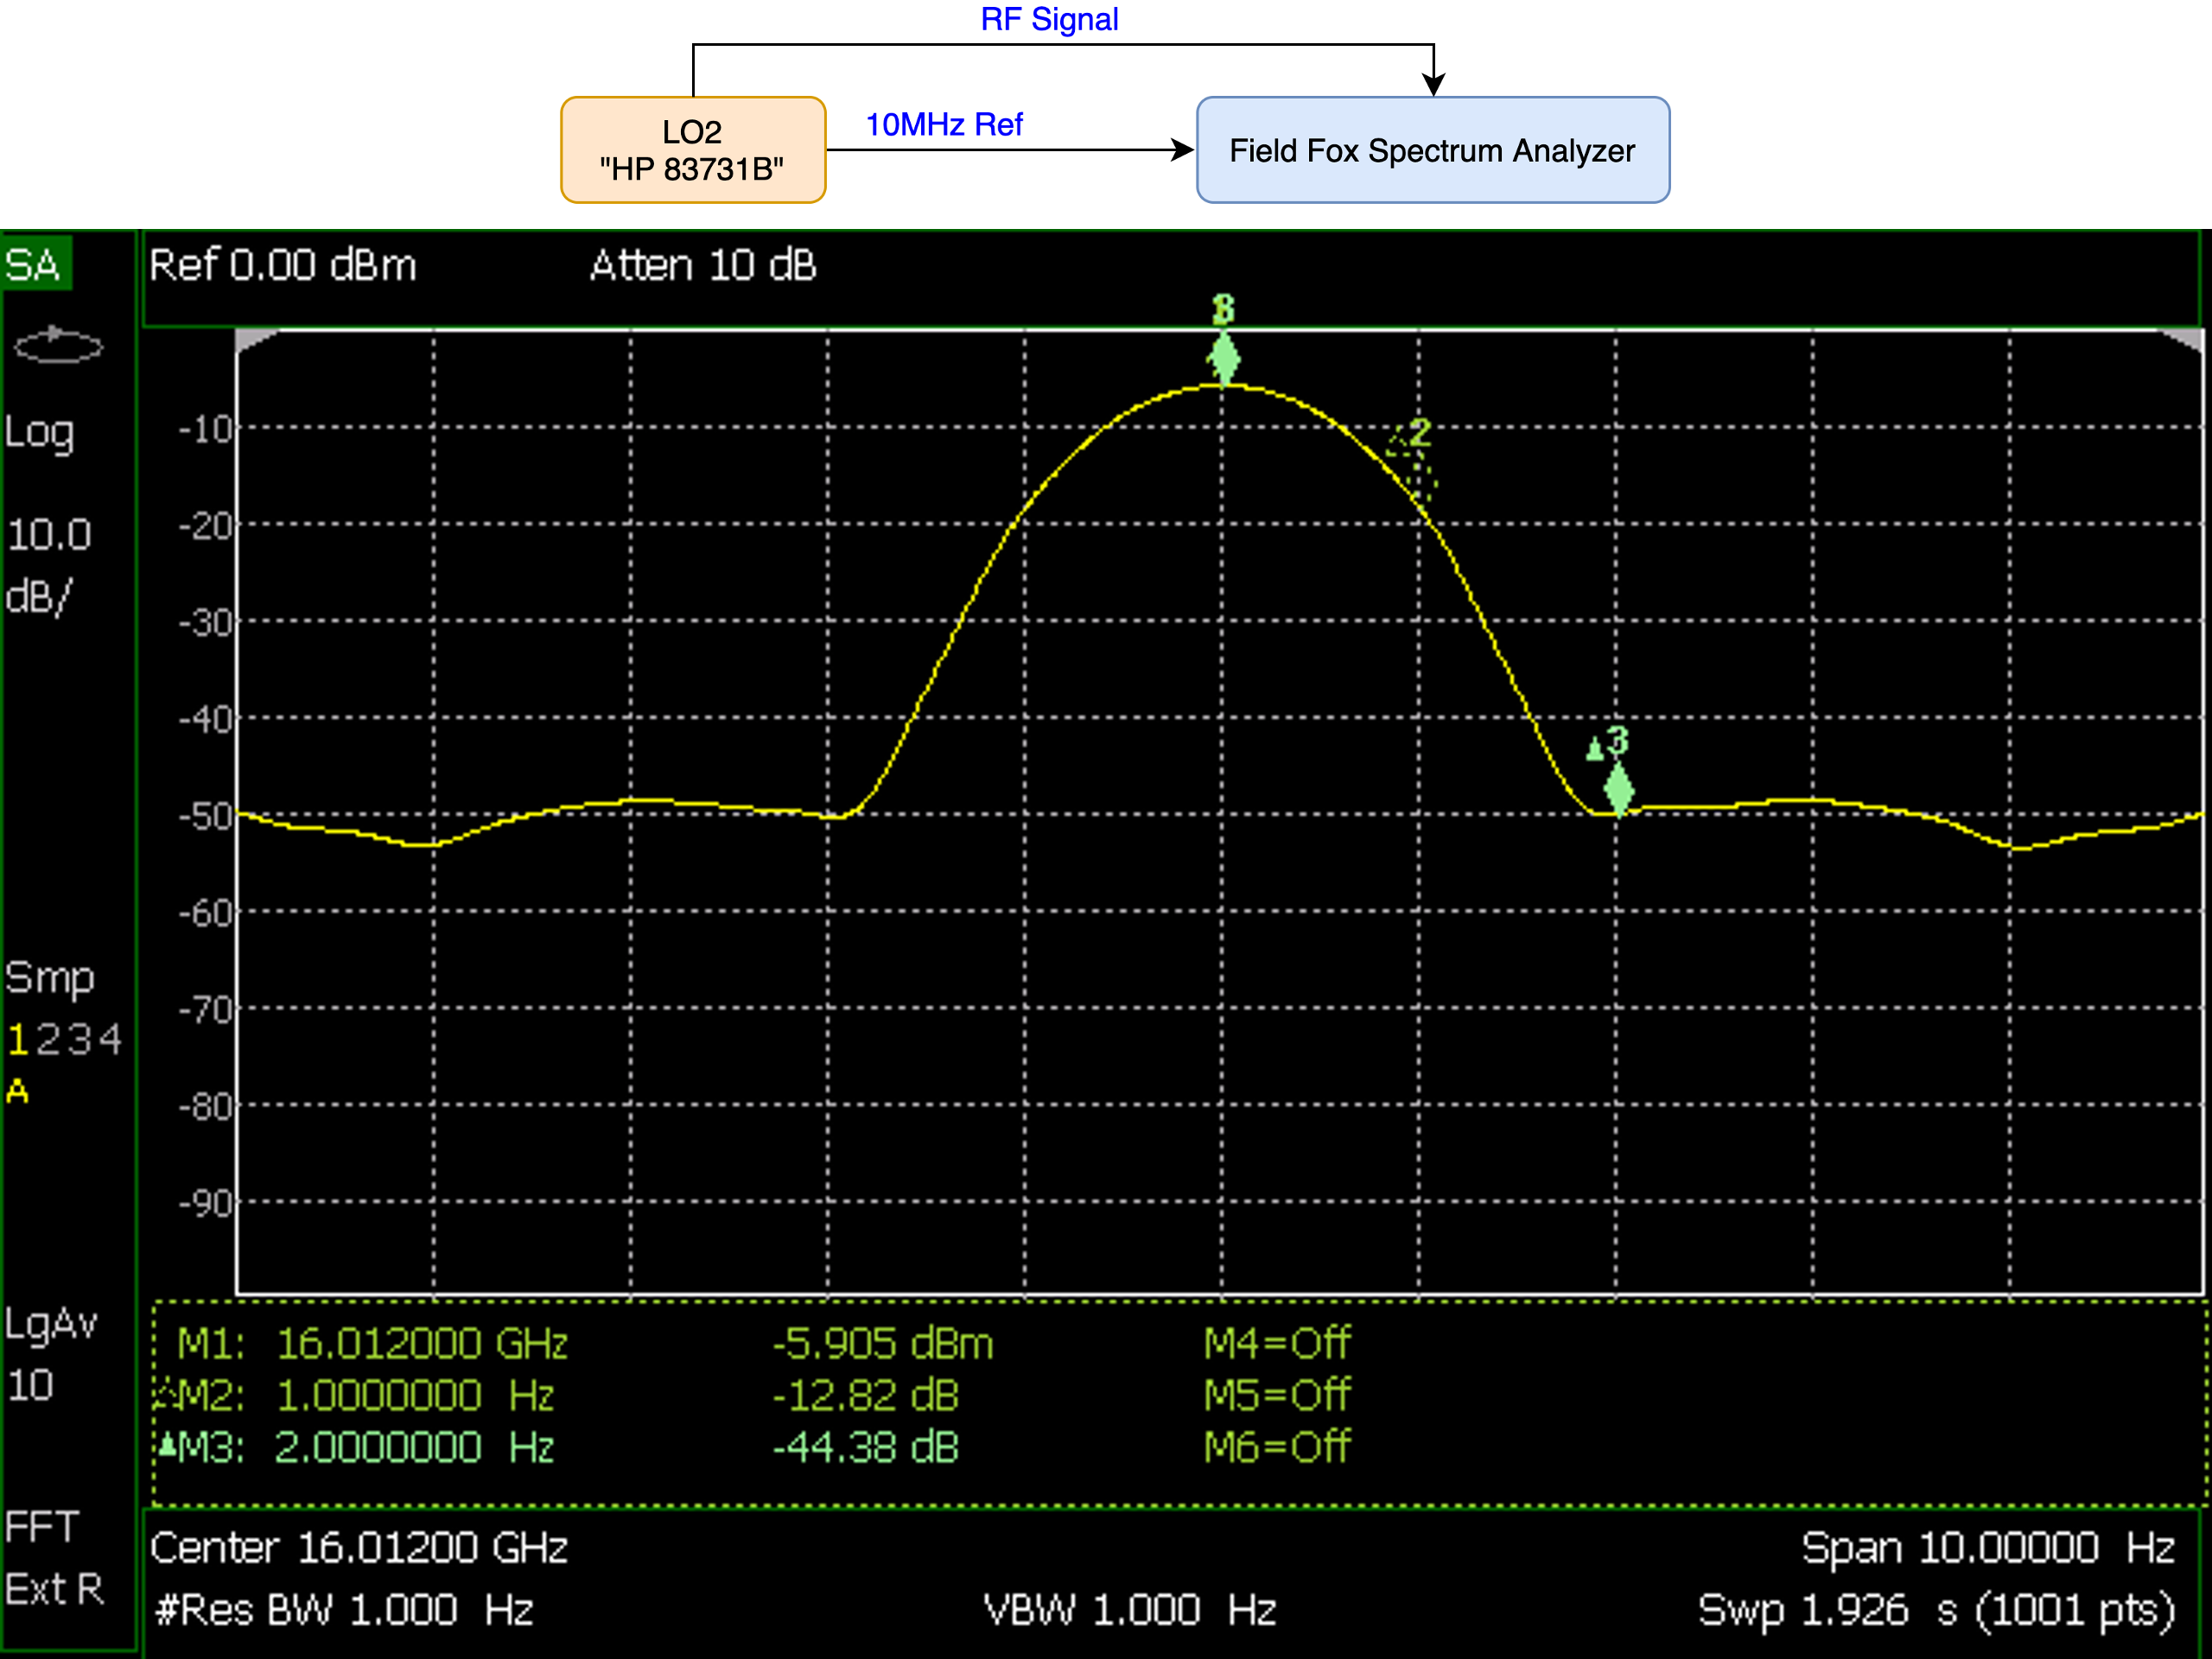
\includegraphics[width=0.8\linewidth]{figures/Measurement-Setup1-LO2-10Hz.png}}
\caption{Narrow band spectra of LO2 with a frequency span of 10\,Hz.}
\label{fig:Measurement-Setup1-LO2-10Hz}
\end{figure}
%

%----------------------------------------------------------------------------------------
%	Final Configuration
%-----------------------------------------------------------------------------------------
%----------------------------------------------------------------------------------------
\section{Time Distribution Configuration and LO Spectra}
\label{sec:4}
% ----------------------------------------------------------------


Based on the information gained throughout the investigation of the phase noise and spur measurements we rewired the 10\,MHz reference distribution entirely.
The final configuration of the HCRO SPR time distribution is shown in Figure \ref{fig:Time-Distribution-HCRO-03-11-2020}. One can see that we supply the 10\,MHz reference for the local oscillators directly form the station clock and daisy chain them through. 
%
\begin{figure}[ht!]
\centering{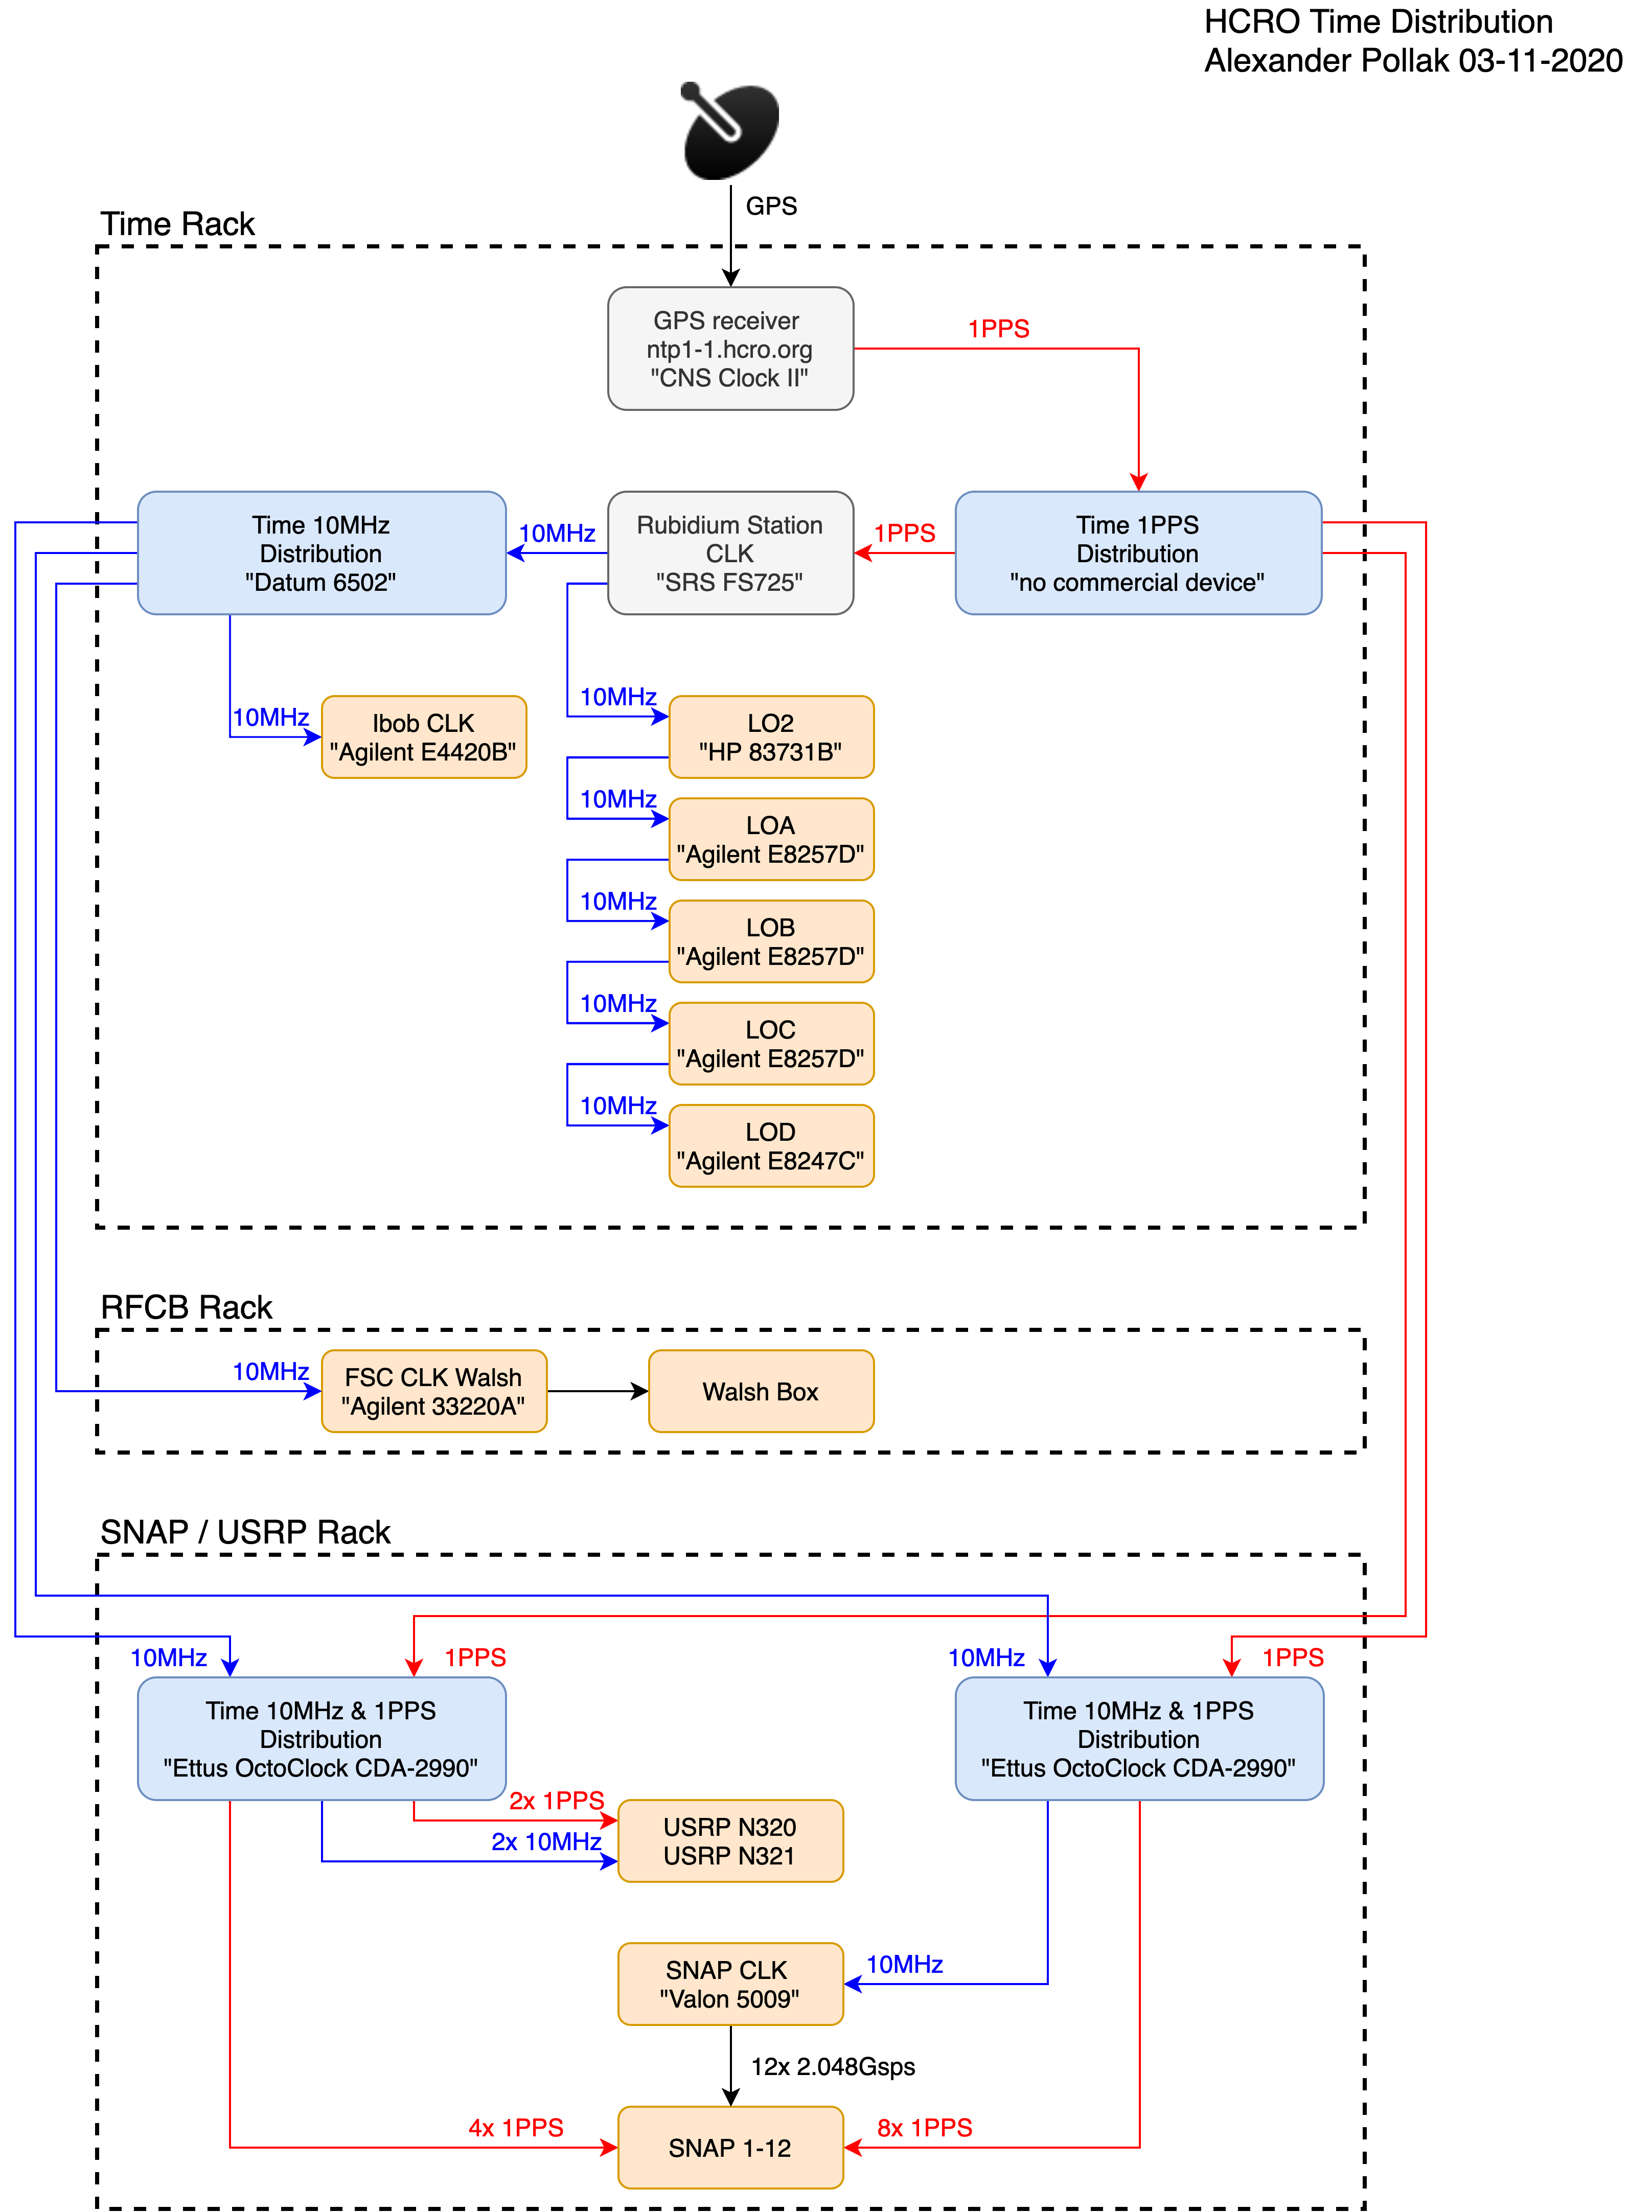
\includegraphics[width=0.8\linewidth]{figures/Time-Distribution-HCRO-03-11-2020.png}}
\caption{Diagram of the HCRO 10\,MHz and 1PPS reference distribution.}
\label{fig:Time-Distribution-HCRO-03-11-2020}
\end{figure}
%
The 10\,MHz reference for all other devices in the SPR is connected to a second 10\,MHz reference output of the station clock and goes through the distribution amplifier. We also want to point out, that the 1PPS provided by the station clock seems to be unreliable. There are records of this clock having this problem in the past, therefore the 1PPS goes first to the 1PPS distribution module and then to the station clock. The spectra of all 5 local oscillators for the final configuration are shown in Figure \ref{fig:10MHZ-TEST-LOA-ALL-CLK} -- \ref{fig:10MHZ-TEST-LOD-ALL-CLK}.

%
\begin{figure}[ht!]
\centering{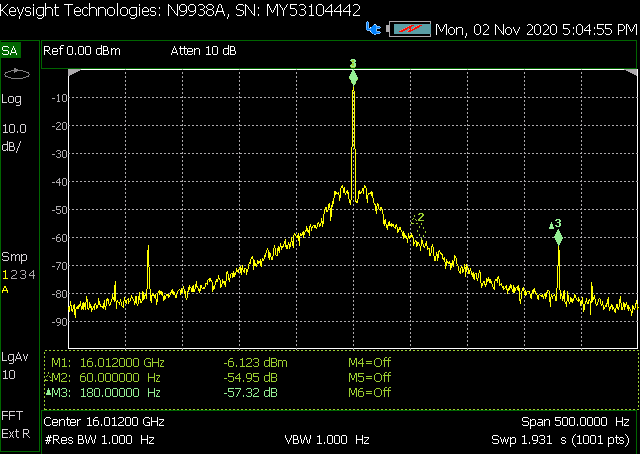
\includegraphics[width=0.8\linewidth]{figures/10MHZ-TEST-LO2-ALL-CLK.png}}
\caption{LO2 spectra for the final configuration as shown in Figure \ref{fig:Time-Distribution-HCRO-03-11-2020}.}
\label{fig:10MHZ-TEST-LOA-ALL-CLK}
\end{figure}
%
%
\begin{figure}[ht!]
\centering{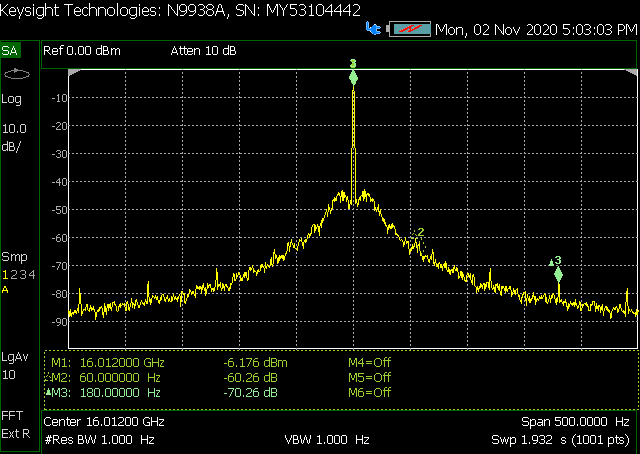
\includegraphics[width=0.8\linewidth]{figures/10MHZ-TEST-LOA-ALL-CLK.png}}
\caption{LOA spectra for the final configuration as shown in Figure \ref{fig:Time-Distribution-HCRO-03-11-2020}.}
\label{fig:10MHZ-TEST-LOA-ALL-CLK}
\end{figure}
%
%
\begin{figure}[ht!]
\centering{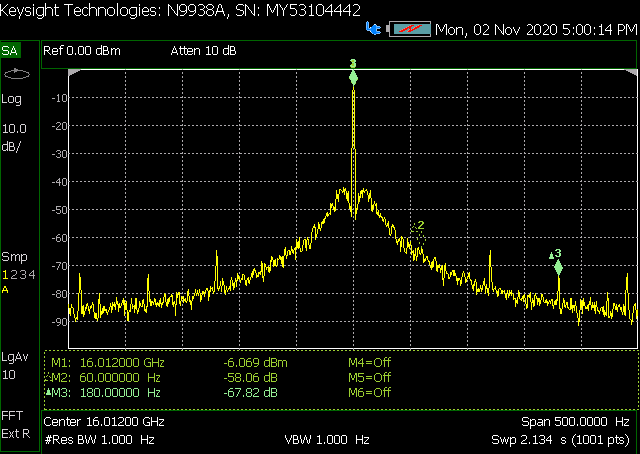
\includegraphics[width=0.8\linewidth]{figures/10MHZ-TEST-LOB-ALL-CLK.png}}
\caption{LOB spectra for the final configuration as shown in Figure \ref{fig:Time-Distribution-HCRO-03-11-2020}.}
\label{fig:10MHZ-TEST-LOB-ALL-CLK}
\end{figure}
%
%
\begin{figure}[ht!]
\centering{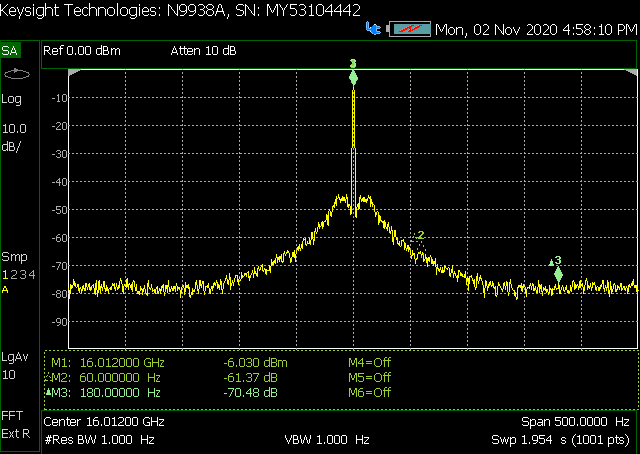
\includegraphics[width=0.8\linewidth]{figures/10MHZ-TEST-LOC-ALL-CLK.png}}
\caption{LOC spectra for the final configuration as shown in Figure \ref{fig:Time-Distribution-HCRO-03-11-2020}.}
\label{fig:10MHZ-TEST-LOC-ALL-CLK}
\end{figure}
%
%
\begin{figure}[ht!]
\centering{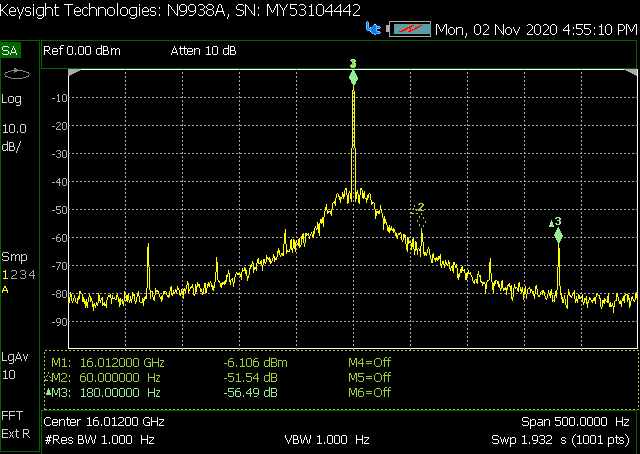
\includegraphics[width=0.8\linewidth]{figures/10MHZ-TEST-LOD-ALL-CLK.png}}
\caption{LOD spectra for the final configuration as shown in Figure \ref{fig:Time-Distribution-HCRO-03-11-2020}.}
\label{fig:10MHZ-TEST-LOD-ALL-CLK}
\end{figure}
%

%----------------------------------------------------------------------------------------
%	BIBLIOGRAPHY
%----------------------------------------------------------------------------------------

%\bibliographystyle{apalike}
%\bibliographystyle{abbrv}
\newpage
\bibliographystyle{apsrev}
\bibliography{bib_memos}

%----------------------------------------------------------------------------------------



\end{document}
